% Options for packages loaded elsewhere
\PassOptionsToPackage{unicode}{hyperref}
\PassOptionsToPackage{hyphens}{url}
\documentclass[
]{article}
\usepackage{xcolor}
\usepackage{amsmath,amssymb}
\setcounter{secnumdepth}{-\maxdimen} % remove section numbering
\usepackage{iftex}
\ifPDFTeX
  \usepackage[T1]{fontenc}
  \usepackage[utf8]{inputenc}
  \usepackage{textcomp} % provide euro and other symbols
\else % if luatex or xetex
  \usepackage{unicode-math} % this also loads fontspec
  \defaultfontfeatures{Scale=MatchLowercase}
  \defaultfontfeatures[\rmfamily]{Ligatures=TeX,Scale=1}
\fi
\usepackage{lmodern}
\ifPDFTeX\else
  % xetex/luatex font selection
\fi
% Use upquote if available, for straight quotes in verbatim environments
\IfFileExists{upquote.sty}{\usepackage{upquote}}{}
\IfFileExists{microtype.sty}{% use microtype if available
  \usepackage[]{microtype}
  \UseMicrotypeSet[protrusion]{basicmath} % disable protrusion for tt fonts
}{}
\makeatletter
\@ifundefined{KOMAClassName}{% if non-KOMA class
  \IfFileExists{parskip.sty}{%
    \usepackage{parskip}
  }{% else
    \setlength{\parindent}{0pt}
    \setlength{\parskip}{6pt plus 2pt minus 1pt}}
}{% if KOMA class
  \KOMAoptions{parskip=half}}
\makeatother
\usepackage{color}
\usepackage{fancyvrb}
\newcommand{\VerbBar}{|}
\newcommand{\VERB}{\Verb[commandchars=\\\{\}]}
\DefineVerbatimEnvironment{Highlighting}{Verbatim}{commandchars=\\\{\}}
% Add ',fontsize=\small' for more characters per line
\newenvironment{Shaded}{}{}
\newcommand{\AlertTok}[1]{\textcolor[rgb]{1.00,0.00,0.00}{\textbf{#1}}}
\newcommand{\AnnotationTok}[1]{\textcolor[rgb]{0.38,0.63,0.69}{\textbf{\textit{#1}}}}
\newcommand{\AttributeTok}[1]{\textcolor[rgb]{0.49,0.56,0.16}{#1}}
\newcommand{\BaseNTok}[1]{\textcolor[rgb]{0.25,0.63,0.44}{#1}}
\newcommand{\BuiltInTok}[1]{\textcolor[rgb]{0.00,0.50,0.00}{#1}}
\newcommand{\CharTok}[1]{\textcolor[rgb]{0.25,0.44,0.63}{#1}}
\newcommand{\CommentTok}[1]{\textcolor[rgb]{0.38,0.63,0.69}{\textit{#1}}}
\newcommand{\CommentVarTok}[1]{\textcolor[rgb]{0.38,0.63,0.69}{\textbf{\textit{#1}}}}
\newcommand{\ConstantTok}[1]{\textcolor[rgb]{0.53,0.00,0.00}{#1}}
\newcommand{\ControlFlowTok}[1]{\textcolor[rgb]{0.00,0.44,0.13}{\textbf{#1}}}
\newcommand{\DataTypeTok}[1]{\textcolor[rgb]{0.56,0.13,0.00}{#1}}
\newcommand{\DecValTok}[1]{\textcolor[rgb]{0.25,0.63,0.44}{#1}}
\newcommand{\DocumentationTok}[1]{\textcolor[rgb]{0.73,0.13,0.13}{\textit{#1}}}
\newcommand{\ErrorTok}[1]{\textcolor[rgb]{1.00,0.00,0.00}{\textbf{#1}}}
\newcommand{\ExtensionTok}[1]{#1}
\newcommand{\FloatTok}[1]{\textcolor[rgb]{0.25,0.63,0.44}{#1}}
\newcommand{\FunctionTok}[1]{\textcolor[rgb]{0.02,0.16,0.49}{#1}}
\newcommand{\ImportTok}[1]{\textcolor[rgb]{0.00,0.50,0.00}{\textbf{#1}}}
\newcommand{\InformationTok}[1]{\textcolor[rgb]{0.38,0.63,0.69}{\textbf{\textit{#1}}}}
\newcommand{\KeywordTok}[1]{\textcolor[rgb]{0.00,0.44,0.13}{\textbf{#1}}}
\newcommand{\NormalTok}[1]{#1}
\newcommand{\OperatorTok}[1]{\textcolor[rgb]{0.40,0.40,0.40}{#1}}
\newcommand{\OtherTok}[1]{\textcolor[rgb]{0.00,0.44,0.13}{#1}}
\newcommand{\PreprocessorTok}[1]{\textcolor[rgb]{0.74,0.48,0.00}{#1}}
\newcommand{\RegionMarkerTok}[1]{#1}
\newcommand{\SpecialCharTok}[1]{\textcolor[rgb]{0.25,0.44,0.63}{#1}}
\newcommand{\SpecialStringTok}[1]{\textcolor[rgb]{0.73,0.40,0.53}{#1}}
\newcommand{\StringTok}[1]{\textcolor[rgb]{0.25,0.44,0.63}{#1}}
\newcommand{\VariableTok}[1]{\textcolor[rgb]{0.10,0.09,0.49}{#1}}
\newcommand{\VerbatimStringTok}[1]{\textcolor[rgb]{0.25,0.44,0.63}{#1}}
\newcommand{\WarningTok}[1]{\textcolor[rgb]{0.38,0.63,0.69}{\textbf{\textit{#1}}}}
\usepackage{longtable,booktabs,array}
\usepackage{calc} % for calculating minipage widths
% Correct order of tables after \paragraph or \subparagraph
\usepackage{etoolbox}
\makeatletter
\patchcmd\longtable{\par}{\if@noskipsec\mbox{}\fi\par}{}{}
\makeatother
% Allow footnotes in longtable head/foot
\IfFileExists{footnotehyper.sty}{\usepackage{footnotehyper}}{\usepackage{footnote}}
\makesavenoteenv{longtable}
\usepackage{graphicx}
\makeatletter
\newsavebox\pandoc@box
\newcommand*\pandocbounded[1]{% scales image to fit in text height/width
  \sbox\pandoc@box{#1}%
  \Gscale@div\@tempa{\textheight}{\dimexpr\ht\pandoc@box+\dp\pandoc@box\relax}%
  \Gscale@div\@tempb{\linewidth}{\wd\pandoc@box}%
  \ifdim\@tempb\p@<\@tempa\p@\let\@tempa\@tempb\fi% select the smaller of both
  \ifdim\@tempa\p@<\p@\scalebox{\@tempa}{\usebox\pandoc@box}%
  \else\usebox{\pandoc@box}%
  \fi%
}
% Set default figure placement to htbp
\def\fps@figure{htbp}
\makeatother
\setlength{\emergencystretch}{3em} % prevent overfull lines
\providecommand{\tightlist}{%
  \setlength{\itemsep}{0pt}\setlength{\parskip}{0pt}}
\usepackage{bookmark}
\IfFileExists{xurl.sty}{\usepackage{xurl}}{} % add URL line breaks if available
\urlstyle{same}
\hypersetup{
  hidelinks,
  pdfcreator={LaTeX via pandoc}}

\author{}
\date{}

\begin{document}

\begin{center}\rule{0.5\linewidth}{0.5pt}\end{center}

📅 \textbf{Date:} 24-02-2025

\begin{center}\rule{0.5\linewidth}{0.5pt}\end{center}

\subsection{\texorpdfstring{\textbf{Session-1: Introduction to Operating
System}}{Session-1: Introduction to Operating System}}\label{session-1-introduction-to-operating-system}

\subsubsection{\texorpdfstring{\textbf{What is an Operating System
(OS)?}}{What is an Operating System (OS)?}}\label{what-is-an-operating-system-os}

An \textbf{Operating System} is \textbf{system software} that
\textbf{manages hardware resources} and provides services for
application software and users. It acts as an \textbf{interface between
users and the hardware}.

\subsubsection{\texorpdfstring{\textbf{Main Functions of an
OS:}}{Main Functions of an OS:}}\label{main-functions-of-an-os}

✅ \textbf{Hardware Manager:} Manages all hardware resources (CPU, RAM,
I/O devices).\\
✅ \textbf{Process Manager:} Supervises tasks/processes/jobs being
executed by the CPU.\\
✅ \textbf{Memory Manager:} Allocates and deallocates memory
dynamically.\\
✅ \textbf{Interface Between User \& Hardware:} Provides a platform for
application execution.

📌 \textbf{Illustration (From Book Reference)}\\
\pandocbounded{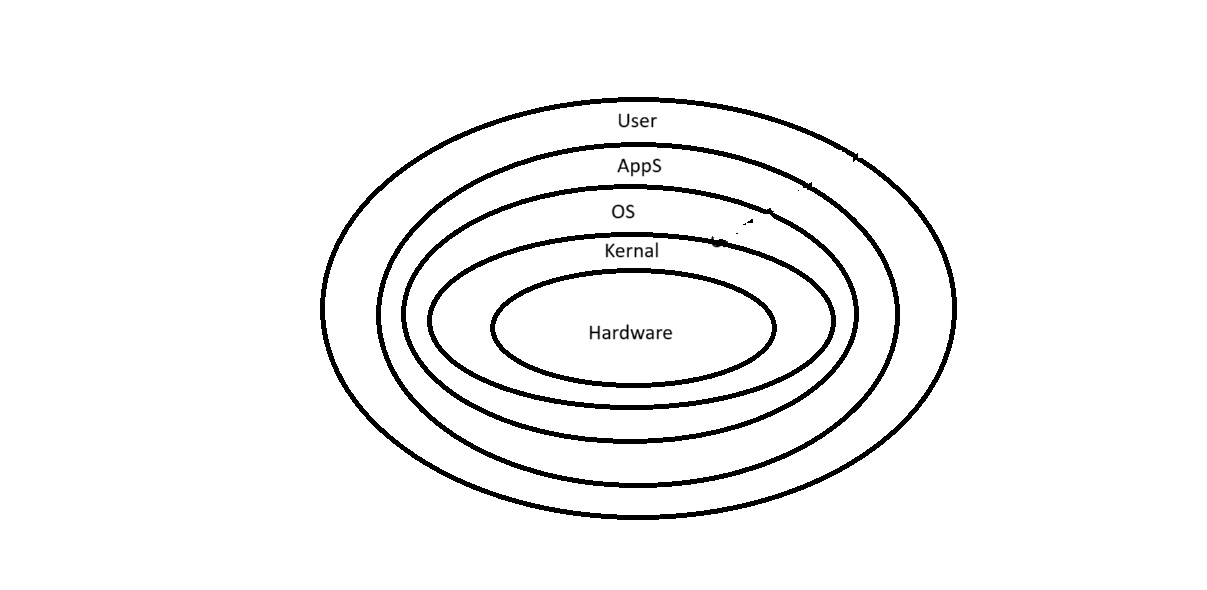
\includegraphics[keepaspectratio]{Day_1_1.jpeg}}

\begin{center}\rule{0.5\linewidth}{0.5pt}\end{center}

\subsubsection{\texorpdfstring{\textbf{How is OS Different from Other
Application
Software?}}{How is OS Different from Other Application Software?}}\label{how-is-os-different-from-other-application-software}

\begin{longtable}[]{@{}
  >{\raggedright\arraybackslash}p{(\linewidth - 4\tabcolsep) * \real{0.3333}}
  >{\raggedright\arraybackslash}p{(\linewidth - 4\tabcolsep) * \real{0.3333}}
  >{\raggedright\arraybackslash}p{(\linewidth - 4\tabcolsep) * \real{0.3333}}@{}}
\toprule\noalign{}
\begin{minipage}[b]{\linewidth}\raggedright
Feature
\end{minipage} & \begin{minipage}[b]{\linewidth}\raggedright
\textbf{Operating System}
\end{minipage} & \begin{minipage}[b]{\linewidth}\raggedright
\textbf{Application Software}
\end{minipage} \\
\midrule\noalign{}
\endhead
\bottomrule\noalign{}
\endlastfoot
\textbf{Installation} & Installed on \textbf{hard drive} & Installed
\textbf{under OS layer} \\
\textbf{Execution} & Runs \textbf{directly on hardware} & Runs
\textbf{on OS} \\
\textbf{Purpose} & Manages system resources & Performs specific user
tasks \\
\textbf{Examples} & Windows, Linux, macOS & MS Word, VLC, Photoshop \\
\end{longtable}

📌 \textbf{Key Point:} \textbf{An application software depends on OS,
but OS does not depend on application software.}

\begin{center}\rule{0.5\linewidth}{0.5pt}\end{center}

\subsubsection{\texorpdfstring{\textbf{Booting
Process}}{Booting Process}}\label{booting-process}

\textbf{Booting} refers to \textbf{loading the OS from the hard drive
into main memory (RAM).}

📌 \textbf{Types of Booting:}

\begin{enumerate}
\def\labelenumi{\arabic{enumi}.}
\tightlist
\item
  \textbf{Cold Booting} → Starting the system from a \textbf{power-off}
  state (\textbf{Initial OS load}).
\item
  \textbf{Hot Booting} → Restarting the system while it's already
  running (\textbf{OS reloads into RAM}).
\end{enumerate}

\begin{center}\rule{0.5\linewidth}{0.5pt}\end{center}

\subsubsection{\texorpdfstring{\textbf{Why is an OS Hardware
Dependent?}}{Why is an OS Hardware Dependent?}}\label{why-is-an-os-hardware-dependent}

📌 \textbf{An OS is hardware-dependent because:}\\
✅ OS interacts with hardware via \textbf{device drivers} specific to
each component.\\
✅ Different hardware architectures (\textbf{x86, ARM, RISC-V}) require
\textbf{compatible OS versions}.\\
✅ Embedded systems require \textbf{customized OS versions} tailored for
performance constraints.

\begin{center}\rule{0.5\linewidth}{0.5pt}\end{center}

\subsubsection{\texorpdfstring{\textbf{Different Components of
OS}}{Different Components of OS}}\label{different-components-of-os}

📌 \textbf{Major OS Components:}

\begin{itemize}
\tightlist
\item
  \textbf{Kernel} → Core system controlling hardware \& processes.
\item
  \textbf{Process Management} → Handles CPU scheduling \& multitasking.
\item
  \textbf{Memory Management} → Allocates RAM efficiently.
\item
  \textbf{File System} → Manages file storage \& retrieval.
\item
  \textbf{Device Management} → Handles I/O devices via drivers.
\item
  \textbf{Security Management} → Protects system data \& access control.
\end{itemize}

📌 \textbf{Illustration:}\\
\pandocbounded{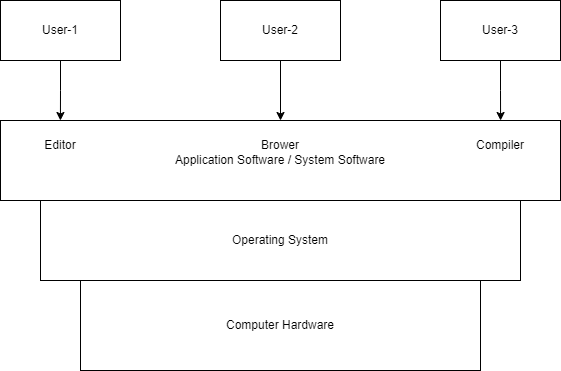
\includegraphics[keepaspectratio]{Day_1_2.png}}

\begin{center}\rule{0.5\linewidth}{0.5pt}\end{center}

\subsubsection{\texorpdfstring{\textbf{Basic Computer Organization
Required for
OS}}{Basic Computer Organization Required for OS}}\label{basic-computer-organization-required-for-os}

📌 \textbf{System Components:}\\
✅ \textbf{CPU} → Executes instructions.\\
✅ \textbf{RAM} → Stores active processes.\\
✅ \textbf{Storage (HDD/SSD)} → Stores OS \& programs.\\
✅ \textbf{I/O Devices} → Keyboard, Mouse, Monitor, Printers.

📌 \textbf{Illustration:}\\
\pandocbounded{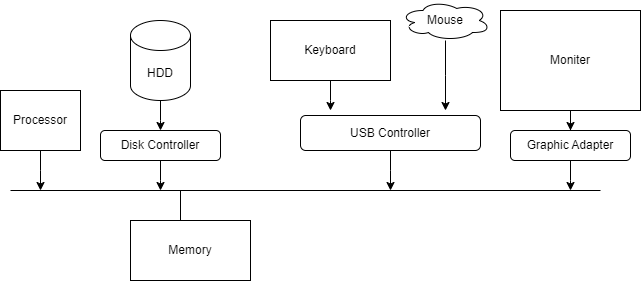
\includegraphics[keepaspectratio]{Day_1_3.png}}

\begin{center}\rule{0.5\linewidth}{0.5pt}\end{center}

\subsubsection{\texorpdfstring{\textbf{Examples of Well-Known Operating
Systems}}{Examples of Well-Known Operating Systems}}\label{examples-of-well-known-operating-systems}

📌 \textbf{Types of OS \& Examples:}

\begin{longtable}[]{@{}
  >{\raggedright\arraybackslash}p{(\linewidth - 4\tabcolsep) * \real{0.3333}}
  >{\raggedright\arraybackslash}p{(\linewidth - 4\tabcolsep) * \real{0.3333}}
  >{\raggedright\arraybackslash}p{(\linewidth - 4\tabcolsep) * \real{0.3333}}@{}}
\toprule\noalign{}
\begin{minipage}[b]{\linewidth}\raggedright
\textbf{Category}
\end{minipage} & \begin{minipage}[b]{\linewidth}\raggedright
\textbf{Examples}
\end{minipage} & \begin{minipage}[b]{\linewidth}\raggedright
\textbf{Description}
\end{minipage} \\
\midrule\noalign{}
\endhead
\bottomrule\noalign{}
\endlastfoot
\textbf{Mobile OS} & Android, iOS & Designed for \textbf{smartphones \&
tablets} \\
\textbf{Embedded OS} & FreeRTOS, VxWorks & Used in \textbf{IoT \&
real-time devices} \\
\textbf{Real-Time OS (RTOS)} & HRT, SRT & Used for
\textbf{mission-critical systems} \\
\textbf{Desktop OS} & Windows, macOS, Chrome OS &
\textbf{General-purpose computing} \\
\textbf{Server OS} & Ubuntu Server, CentOS, Windows Server & Manages
\textbf{network services \& databases} \\
\end{longtable}

📌 \textbf{To-Do:} \textbf{``How are these OS types different from each
other?''}

\begin{center}\rule{0.5\linewidth}{0.5pt}\end{center}

\subsubsection{\texorpdfstring{\textbf{Functions of an
OS}}{Functions of an OS}}\label{functions-of-an-os}

📌 \textbf{Core OS Functionalities:}

✅ \textbf{Process Management}

\begin{itemize}
\tightlist
\item
  \textbf{Handles CPU scheduling} (e.g., FCFS, SJF, Round Robin).
\item
  Ensures smooth multitasking.
\item
  \textbf{Illustration:}\\
  \pandocbounded{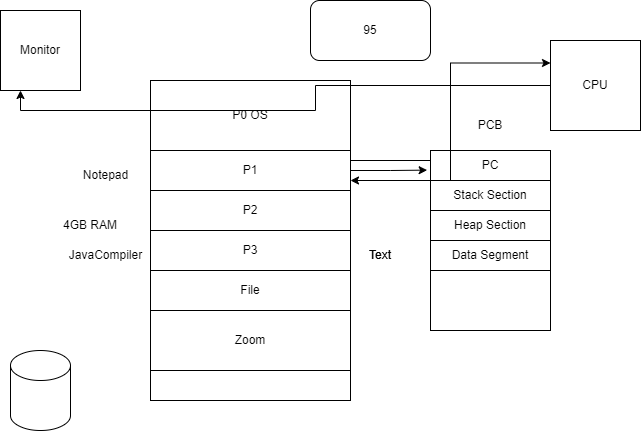
\includegraphics[keepaspectratio]{Day_1_4.png}}
\end{itemize}

✅ \textbf{Memory Management}

\begin{itemize}
\tightlist
\item
  Allocates memory to processes dynamically.
\item
  Uses \textbf{paging \& segmentation}.
\end{itemize}

✅ \textbf{Device Management}

\begin{itemize}
\tightlist
\item
  Manages hardware devices via \textbf{device drivers}.
\end{itemize}

✅ \textbf{Disk Management}

\begin{itemize}
\tightlist
\item
  Organizes data using \textbf{file systems (NTFS, FAT32, ext4)}.
\end{itemize}

✅ \textbf{Security Management}

\begin{itemize}
\tightlist
\item
  Includes \textbf{firewalls, antivirus, authentication}.
\end{itemize}

\begin{center}\rule{0.5\linewidth}{0.5pt}\end{center}

\subsubsection{\texorpdfstring{\textbf{Topics for
Tomorrow:}}{Topics for Tomorrow:}}\label{topics-for-tomorrow}

📌 \textbf{Upcoming Topics:}

\begin{itemize}
\tightlist
\item
  \textbf{User \& Kernel Space}
\item
  \textbf{Interrupts \& System Calls}
\item
  \textbf{Memory Hierarchy in Computers}
\item
  \textbf{Types of OS (Batch, Time-Sharing, Real-Time, etc.)}
\end{itemize}

\begin{center}\rule{0.5\linewidth}{0.5pt}\end{center}

\subsection{\texorpdfstring{\textbf{Session-2: Introduction to
Linux}}{Session-2: Introduction to Linux}}\label{session-2-introduction-to-linux}

\subsubsection{\texorpdfstring{\textbf{What is
Linux?}}{What is Linux?}}\label{what-is-linux}

📌 \textbf{Linux is an open-source OS}, meaning its source code is
available for modification.

\begin{itemize}
\tightlist
\item
  Developed by \textbf{Linus Torvalds in 1991}.
\item
  Backed by an \textbf{open-source community} for continuous updates.
\end{itemize}

\begin{center}\rule{0.5\linewidth}{0.5pt}\end{center}

\subsubsection{\texorpdfstring{\textbf{Features of
Linux}}{Features of Linux}}\label{features-of-linux}

✅ \textbf{No Cost / Low Cost} → Free to use.\\
✅ \textbf{Multi-Tasking} → Supports \textbf{multiple processes} at
once.\\
✅ \textbf{Security} → Built-in \textbf{permissions \& encryption}.\\
✅ \textbf{Customizable} → Users can modify \textbf{kernel \&
utilities}.\\
✅ \textbf{Multi-User} → Supports \textbf{multiple users on the same
system}.\\
✅ \textbf{Better File System} → Supports \textbf{ext4, XFS, Btrfs}.\\
✅ \textbf{CLI \& GUI Support} → Terminal-based \& graphical interfaces.

\begin{center}\rule{0.5\linewidth}{0.5pt}\end{center}

\subsubsection{\texorpdfstring{\textbf{Linux File System
Hierarchy}}{Linux File System Hierarchy}}\label{linux-file-system-hierarchy}

📌 \textbf{Directory Structure in Linux:}

\begin{longtable}[]{@{}ll@{}}
\toprule\noalign{}
\textbf{Directory} & \textbf{Description} \\
\midrule\noalign{}
\endhead
\bottomrule\noalign{}
\endlastfoot
\texttt{/} & \textbf{Root directory} (Base of the filesystem) \\
\texttt{/bin} & Contains \textbf{user binaries} (e.g., \texttt{ls},
\texttt{cp}, \texttt{mv}) \\
\texttt{/sbin} & Stores \textbf{system binaries} (e.g., \texttt{fdisk},
\texttt{fsck}) \\
\texttt{/etc} & Contains \textbf{configuration files} (e.g.,
\texttt{passwd}, \texttt{hosts}) \\
\texttt{/dev} & Stores \textbf{device files} (e.g., \texttt{/dev/sda}
for disks) \\
\texttt{/proc} & Holds \textbf{process info} (e.g.,
\texttt{/proc/cpuinfo}) \\
\texttt{/var} & Stores \textbf{log \& cache files} \\
\texttt{/tmp} & Temporary files (Deleted on reboot) \\
\texttt{/usr} & User-related files \& programs \\
\texttt{/home} & \textbf{User home directories}
(\texttt{/home/user1}) \\
\texttt{/log} & Stores \textbf{system logs} (May vary across
distributions) \\
\end{longtable}

\begin{center}\rule{0.5\linewidth}{0.5pt}\end{center}

\subsubsection{\texorpdfstring{\textbf{Basic Linux
Commands}}{Basic Linux Commands}}\label{basic-linux-commands}

📌 \textbf{File \& Directory Commands:}

\begin{itemize}
\tightlist
\item
  \texttt{ls} → List files \& directories
\item
  \texttt{cd\ \textless{}dir\textgreater{}} → Change directory
\item
  \texttt{mkdir\ \textless{}dir\textgreater{}} → Create a directory
\item
  \texttt{rm\ \textless{}file\textgreater{}} → Remove a file
\item
  \texttt{rmdir\ \textless{}dir\textgreater{}} → Remove a directory
\end{itemize}

📌 \textbf{Operators in Linux:}

\begin{enumerate}
\def\labelenumi{\arabic{enumi}.}
\item
  \textbf{Redirection (\texttt{\textgreater{}},
  \texttt{\textgreater{}\textgreater{}})}

  \begin{itemize}
  \tightlist
  \item
    \texttt{echo\ "Hello"\ \textgreater{}\ file.txt} → Write to file
  \item
    \texttt{echo\ "World"\ \textgreater{}\textgreater{}\ file.txt} →
    Append to file
  \end{itemize}
\item
  \textbf{Pipe (\texttt{\textbar{}})}

  \begin{itemize}
  \tightlist
  \item
    \texttt{cat\ file.txt\ \textbar{}\ grep\ "error"} → Filters output
  \end{itemize}
\end{enumerate}

\section{\texorpdfstring{\textbf{OS Notes -- Day
2}}{OS Notes -- Day 2}}\label{os-notes-day-2}

📅 \textbf{Date:} 26-02-2025

\subsubsection{Session 1}\label{session-1}

\subsection{\texorpdfstring{\textbf{OS Introduction and Basic
Functions}}{OS Introduction and Basic Functions}}\label{os-introduction-and-basic-functions}

\subsubsection{\texorpdfstring{\textbf{User and Kernel Space \&
Mode}}{User and Kernel Space \& Mode}}\label{user-and-kernel-space-mode}

📌 \textbf{Definition:}

\begin{itemize}
\tightlist
\item
  \textbf{User Space:} Runs user applications with \textbf{restricted
  access} to hardware.
\item
  \textbf{Kernel Space:} Executes \textbf{OS services and device
  drivers} with \textbf{full system access}.
\end{itemize}

📌 \textbf{Modes:}

\begin{itemize}
\tightlist
\item
  \textbf{User Mode:}

  \begin{itemize}
  \tightlist
  \item
    Runs normal applications (\textbf{text editors, browsers, media
    players}).
  \item
    Cannot directly access hardware resources.
  \end{itemize}
\item
  \textbf{Kernel Mode:}

  \begin{itemize}
  \tightlist
  \item
    Runs \textbf{OS core functions, device drivers, and memory
    management}.
  \item
    Has \textbf{full privileges} over CPU, memory, and hardware.
  \end{itemize}
\end{itemize}

📌 \textbf{Illustration:}\\
\pandocbounded{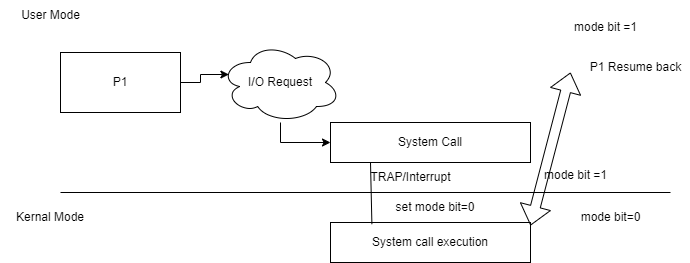
\includegraphics[keepaspectratio]{Day_2_2.png}}

\begin{center}\rule{0.5\linewidth}{0.5pt}\end{center}

\subsubsection{\texorpdfstring{\textbf{Interrupts and System
Calls}}{Interrupts and System Calls}}\label{interrupts-and-system-calls}

📌 \textbf{Interrupts:}\\
Interrupts \textbf{pause CPU execution} to handle critical events (e.g.,
keyboard input, disk I/O).

📌 \textbf{System Calls:}\\
System calls act as a \textbf{bridge between user applications and the
OS kernel}.

📌 \textbf{Types of System Calls:}

\begin{longtable}[]{@{}
  >{\raggedright\arraybackslash}p{(\linewidth - 4\tabcolsep) * \real{0.3333}}
  >{\raggedright\arraybackslash}p{(\linewidth - 4\tabcolsep) * \real{0.3333}}
  >{\raggedright\arraybackslash}p{(\linewidth - 4\tabcolsep) * \real{0.3333}}@{}}
\toprule\noalign{}
\begin{minipage}[b]{\linewidth}\raggedright
\textbf{Category}
\end{minipage} & \begin{minipage}[b]{\linewidth}\raggedright
\textbf{System Calls}
\end{minipage} & \begin{minipage}[b]{\linewidth}\raggedright
\textbf{Description}
\end{minipage} \\
\midrule\noalign{}
\endhead
\bottomrule\noalign{}
\endlastfoot
\textbf{File Management} & \texttt{open()}, \texttt{close()},
\texttt{read()}, \texttt{write()}, \texttt{delete()} & Operations on
files \\
\textbf{Process Control} & \texttt{fork()}, \texttt{wait()},
\texttt{exec()}, \texttt{exit()} & Process creation and execution \\
\textbf{Device Management} & \texttt{ioctl()}, \texttt{read()},
\texttt{write()} & Communicate with hardware devices \\
\textbf{Information Retrieval} & \texttt{getpid()}, \texttt{sysinfo()} &
Retrieve system data \\
\textbf{IPC (Inter-Process Communication)} & \texttt{wait()},
\texttt{notify()} & Process communication \\
\end{longtable}

Example:

\begin{Shaded}
\begin{Highlighting}[]
\PreprocessorTok{\#include }\ImportTok{\textless{}stdio.h\textgreater{}}
\PreprocessorTok{\#include }\ImportTok{\textless{}unistd.h\textgreater{}}
\DataTypeTok{int}\NormalTok{ main}\OperatorTok{()} \OperatorTok{\{}
\NormalTok{    printf}\OperatorTok{(}\StringTok{"Process ID: }\SpecialCharTok{\%d\textbackslash{}n}\StringTok{"}\OperatorTok{,}\NormalTok{ getpid}\OperatorTok{());}  \CommentTok{// Get process ID using system call}
    \ControlFlowTok{return} \DecValTok{0}\OperatorTok{;}
\OperatorTok{\}}
\end{Highlighting}
\end{Shaded}

\begin{center}\rule{0.5\linewidth}{0.5pt}\end{center}

\subsection{\texorpdfstring{\textbf{Types of Operating
Systems}}{Types of Operating Systems}}\label{types-of-operating-systems}

📌 \textbf{Major OS Types:}

\begin{longtable}[]{@{}
  >{\raggedright\arraybackslash}p{(\linewidth - 4\tabcolsep) * \real{0.3333}}
  >{\raggedright\arraybackslash}p{(\linewidth - 4\tabcolsep) * \real{0.3333}}
  >{\raggedright\arraybackslash}p{(\linewidth - 4\tabcolsep) * \real{0.3333}}@{}}
\toprule\noalign{}
\begin{minipage}[b]{\linewidth}\raggedright
\textbf{Type}
\end{minipage} & \begin{minipage}[b]{\linewidth}\raggedright
\textbf{Description}
\end{minipage} & \begin{minipage}[b]{\linewidth}\raggedright
\textbf{Example}
\end{minipage} \\
\midrule\noalign{}
\endhead
\bottomrule\noalign{}
\endlastfoot
\textbf{Batch OS} & Executes jobs in batches, no user interaction & IBM
OS/360 \\
\textbf{Multiprogramming OS} & Runs multiple processes simultaneously &
UNIX \\
\textbf{Multitasking OS} & Allows multiple applications to run at the
same time & Windows, macOS \\
\textbf{Multiprocessing OS} & Uses multiple CPUs for parallel execution
& Linux, Unix \\
\textbf{Clustered OS} & Manages multiple computers as one system &
Google Cloud OS \\
\textbf{Distributed OS} & Spreads processing tasks across networked
computers & Amoeba OS \\
\textbf{Embedded OS} & Runs on \textbf{specialized devices} (low
resource usage) & FreeRTOS, QNX \\
\end{longtable}

📌 \textbf{Illustration:}\\
\pandocbounded{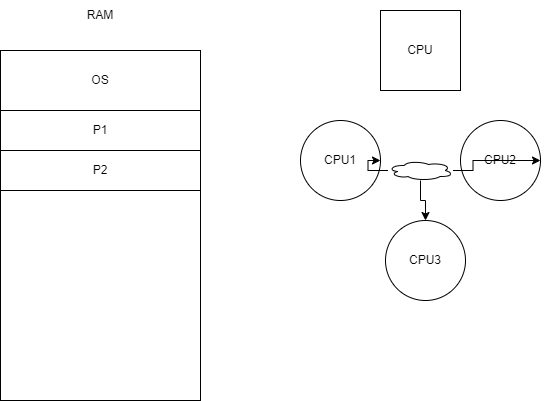
\includegraphics[keepaspectratio]{Day_2_1.png}}

\begin{center}\rule{0.5\linewidth}{0.5pt}\end{center}

\subsection{\texorpdfstring{\textbf{Process
Management}}{Process Management}}\label{process-management}

📌 \textbf{Definition:}\\
A \textbf{process} is a program \textbf{loaded into RAM for execution}.

📌 \textbf{Process Types:}

\begin{itemize}
\tightlist
\item
  \textbf{Preemptive Process:} Can be \textbf{interrupted} and resumed
  later.
\item
  \textbf{Non-Preemptive Process:} Runs \textbf{without interruption}
  until completion.
\end{itemize}

📌 \textbf{Process Control Block (PCB):}\\
Each process has a \textbf{PCB} storing:\\
✅ \textbf{Process ID}\\
✅ \textbf{State (Ready, Running, Blocked, etc.)}\\
✅ \textbf{Program Counter}\\
✅ \textbf{CPU Registers}

📌 \textbf{Illustration:}\\
\pandocbounded{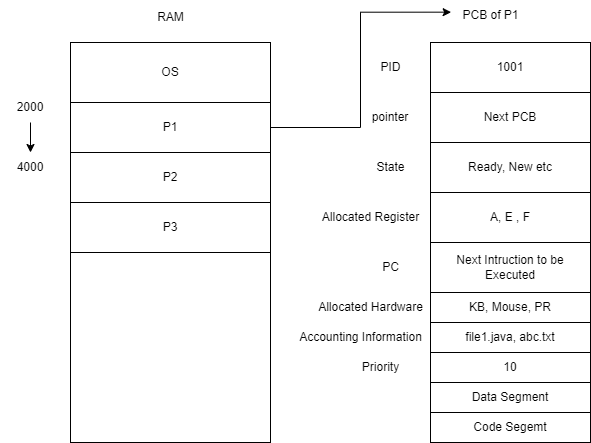
\includegraphics[keepaspectratio]{Day_2_3.png}}

\begin{center}\rule{0.5\linewidth}{0.5pt}\end{center}

\subsubsection{\texorpdfstring{\textbf{Process Life
Cycle}}{Process Life Cycle}}\label{process-life-cycle}

📌 \textbf{Five States of a Process:}\\
1️⃣ \textbf{New} → Process is created.\\
2️⃣ \textbf{Ready} → Waiting for CPU allocation.\\
3️⃣ \textbf{Running} → Currently executing instructions.\\
4️⃣ \textbf{Blocked} → Waiting for I/O completion.\\
5️⃣ \textbf{Terminated} → Process execution finishes.

📌 \textbf{Illustration:}\\
\pandocbounded{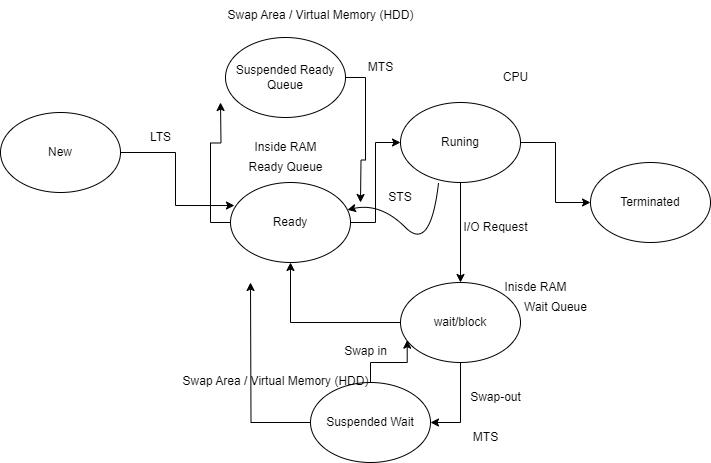
\includegraphics[keepaspectratio]{Day_2_4.png}}

\begin{center}\rule{0.5\linewidth}{0.5pt}\end{center}

\subsubsection{\texorpdfstring{\textbf{Schedulers \& Scheduling
Algorithms}}{Schedulers \& Scheduling Algorithms}}\label{schedulers-scheduling-algorithms}

📌 \textbf{Schedulers:}

\begin{itemize}
\tightlist
\item
  \textbf{Short-Term Scheduler} → Selects process for CPU execution.
\item
  \textbf{Medium-Term Scheduler} → Swaps processes between RAM and disk.
\item
  \textbf{Long-Term Scheduler} → Controls which processes \textbf{enter
  the system}.
\end{itemize}

📌 \textbf{Scheduling Algorithms:}

1️⃣ \textbf{FCFS (First Come First Serve):}

\begin{itemize}
\tightlist
\item
  Executes processes \textbf{in order of arrival}.
\item
  \textbf{Non-preemptive} (Once started, it runs until completion).
\end{itemize}

📌 \textbf{Illustration:}\\
\pandocbounded{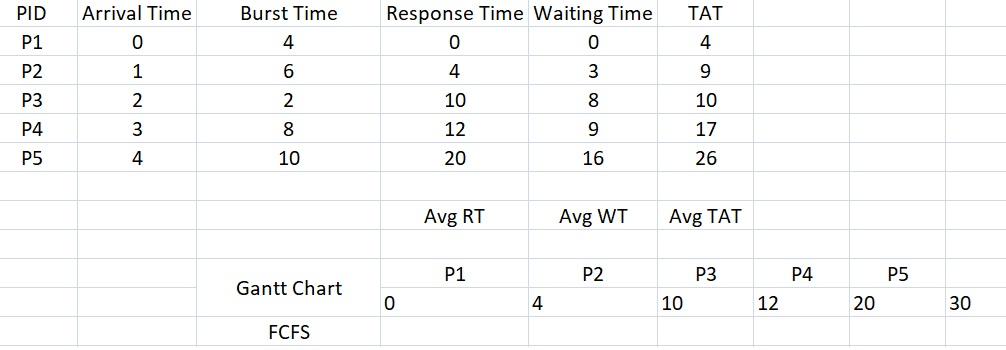
\includegraphics[keepaspectratio]{Day_2_5.png}}

\begin{longtable}[]{@{}
  >{\raggedright\arraybackslash}p{(\linewidth - 0\tabcolsep) * \real{0.0556}}@{}}
\toprule\noalign{}
\endhead
\bottomrule\noalign{}
\endlastfoot
\# \textbf{Schedulers \& Scheduling Algorithms -- Detailed
Explanation} \\
Schedulers and scheduling algorithms are \textbf{essential for process
management} in an operating system. They determine \textbf{which process
gets the CPU and for how long}, ensuring efficient execution of multiple
processes. \\
\end{longtable}

\subsection{\texorpdfstring{\textbf{1️⃣ What is a
Scheduler?}}{1️⃣ What is a Scheduler?}}\label{what-is-a-scheduler}

A \textbf{scheduler} is a system component that manages \textbf{process
execution} by selecting which process runs next. The OS contains
\textbf{three types of schedulers}, each responsible for different
stages of process execution.

📌 \textbf{Three Types of Schedulers:}

\begin{longtable}[]{@{}
  >{\raggedright\arraybackslash}p{(\linewidth - 6\tabcolsep) * \real{0.2500}}
  >{\raggedright\arraybackslash}p{(\linewidth - 6\tabcolsep) * \real{0.2500}}
  >{\raggedright\arraybackslash}p{(\linewidth - 6\tabcolsep) * \real{0.2500}}
  >{\raggedright\arraybackslash}p{(\linewidth - 6\tabcolsep) * \real{0.2500}}@{}}
\toprule\noalign{}
\begin{minipage}[b]{\linewidth}\raggedright
\textbf{Scheduler}
\end{minipage} & \begin{minipage}[b]{\linewidth}\raggedright
\textbf{Function}
\end{minipage} & \begin{minipage}[b]{\linewidth}\raggedright
\textbf{Affects Which States?}
\end{minipage} & \begin{minipage}[b]{\linewidth}\raggedright
\textbf{Frequency of Execution}
\end{minipage} \\
\midrule\noalign{}
\endhead
\bottomrule\noalign{}
\endlastfoot
\textbf{Long-Term Scheduler (Job Scheduler)} & Decides which processes
\textbf{enter the ready queue} from the new state & \emph{New → Ready} &
\textbf{Low (Seconds/Minutes)} \\
\textbf{Short-Term Scheduler (CPU Scheduler)} & Selects which process
\textbf{runs on the CPU} next & \emph{Ready → Running} & \textbf{Very
High (Milliseconds)} \\
\textbf{Medium-Term Scheduler (Swapper)} & Swaps processes \textbf{in
and out of RAM} to optimize memory usage & \emph{Running/Blocked →
Suspended} & \textbf{Medium (Seconds)} \\
\end{longtable}

\begin{center}\rule{0.5\linewidth}{0.5pt}\end{center}

\subsubsection{\texorpdfstring{\textbf{📍 1. Long-Term Scheduler (Job
Scheduler)}}{📍 1. Long-Term Scheduler (Job Scheduler)}}\label{long-term-scheduler-job-scheduler}

\begin{itemize}
\tightlist
\item
  \textbf{Function:} Controls \textbf{which processes are admitted} into
  the system for execution.
\item
  \textbf{Key Role:} Regulates the \textbf{degree of multiprogramming}
  (number of processes in memory).
\item
  \textbf{If Too Many Processes:} System may slow down due to
  \textbf{overloaded memory}.
\item
  \textbf{If Too Few Processes:} CPU remains \textbf{idle}, leading to
  \textbf{poor resource utilization}.
\item
  \textbf{Example:} A user starts \textbf{multiple programs} (browser,
  video player, text editor). The OS decides \textbf{which ones enter
  RAM} based on availability.
\end{itemize}

📌 \textbf{Effect on Process Life Cycle:}

\begin{itemize}
\tightlist
\item
  \textbf{New → Ready} (Moves selected processes to memory).
\end{itemize}

\begin{center}\rule{0.5\linewidth}{0.5pt}\end{center}

\subsubsection{\texorpdfstring{\textbf{📍 2. Short-Term Scheduler (CPU
Scheduler)}}{📍 2. Short-Term Scheduler (CPU Scheduler)}}\label{short-term-scheduler-cpu-scheduler}

\begin{itemize}
\tightlist
\item
  \textbf{Function:} Decides \textbf{which process gets CPU time} from
  the \textbf{ready queue}.
\item
  \textbf{Key Role:} Ensures that processes \textbf{execute
  efficiently}.
\item
  \textbf{Executes Frequently:} Runs \textbf{every few milliseconds} to
  switch processes rapidly.
\item
  \textbf{Example:} If you're playing music while using a web browser,
  the CPU scheduler \textbf{switches tasks} between them rapidly, making
  it seem like both run simultaneously.
\end{itemize}

📌 \textbf{Effect on Process Life Cycle:}

\begin{itemize}
\tightlist
\item
  \textbf{Ready → Running} (Selects process for CPU execution).
\item
  \textbf{Running → Ready} (If preempted, moves back to ready queue).
\end{itemize}

\begin{center}\rule{0.5\linewidth}{0.5pt}\end{center}

\subsubsection{\texorpdfstring{\textbf{📍 3. Medium-Term Scheduler
(Swapper)}}{📍 3. Medium-Term Scheduler (Swapper)}}\label{medium-term-scheduler-swapper}

\begin{itemize}
\tightlist
\item
  \textbf{Function:} Swaps processes between \textbf{RAM and disk} to
  manage memory efficiently.
\item
  \textbf{Key Role:} Helps \textbf{free up RAM} when memory is full.
\item
  \textbf{Example:} If a \textbf{background process} (e.g., a minimized
  browser tab) is \textbf{inactive}, the OS moves it to the \textbf{swap
  area on disk}. It gets \textbf{restored} when needed.
\end{itemize}

📌 \textbf{Effect on Process Life Cycle:}

\begin{itemize}
\tightlist
\item
  \textbf{Running/Blocked → Suspended} (Moves process to disk).
\item
  \textbf{Suspended → Ready} (Brings it back when memory is available).
\end{itemize}

\begin{center}\rule{0.5\linewidth}{0.5pt}\end{center}

\subsection{\texorpdfstring{\textbf{2️⃣ What is a Scheduling
Algorithm?}}{2️⃣ What is a Scheduling Algorithm?}}\label{what-is-a-scheduling-algorithm}

A \textbf{scheduling algorithm} determines \textbf{how the CPU is
assigned to processes} in the ready queue.

📌 \textbf{Objectives of CPU Scheduling:}\\
✅ \textbf{Maximize CPU Utilization} → Keep CPU \textbf{busy}.\\
✅ \textbf{Minimize Waiting Time} → Reduce time spent \textbf{waiting}
in the ready queue.\\
✅ \textbf{Minimize Turnaround Time} → Shorten \textbf{total process
execution time}.\\
✅ \textbf{Ensure Fairness} → Every process \textbf{gets CPU time}.

📌 \textbf{Scheduling Algorithms are divided into:}

\begin{itemize}
\tightlist
\item
  \textbf{Non-Preemptive:} Once a process starts executing, it
  \textbf{cannot be interrupted} until it finishes.
\item
  \textbf{Preemptive:} A process \textbf{can be interrupted} and moved
  back to the ready queue if a higher-priority process arrives.
\end{itemize}

\begin{center}\rule{0.5\linewidth}{0.5pt}\end{center}

\subsection{\texorpdfstring{\textbf{3️⃣ CPU Scheduling Algorithms (With
Examples \&
Diagrams)}}{3️⃣ CPU Scheduling Algorithms (With Examples \& Diagrams)}}\label{cpu-scheduling-algorithms-with-examples-diagrams}

\subsubsection{\texorpdfstring{\textbf{🔹 1. First Come, First Serve
(FCFS) --
Non-Preemptive}}{🔹 1. First Come, First Serve (FCFS) -- Non-Preemptive}}\label{first-come-first-serve-fcfs-non-preemptive}

\begin{itemize}
\tightlist
\item
  \textbf{Processes are scheduled based on arrival time (FIFO -- First
  In, First Out).}
\item
  \textbf{Disadvantage:} Causes \textbf{convoy effect} -- a short job
  waits for a long job to finish.
\end{itemize}

📌 \textbf{Example:}

\begin{longtable}[]{@{}
  >{\raggedright\arraybackslash}p{(\linewidth - 10\tabcolsep) * \real{0.1667}}
  >{\raggedright\arraybackslash}p{(\linewidth - 10\tabcolsep) * \real{0.1667}}
  >{\raggedright\arraybackslash}p{(\linewidth - 10\tabcolsep) * \real{0.1667}}
  >{\raggedright\arraybackslash}p{(\linewidth - 10\tabcolsep) * \real{0.1667}}
  >{\raggedright\arraybackslash}p{(\linewidth - 10\tabcolsep) * \real{0.1667}}
  >{\raggedright\arraybackslash}p{(\linewidth - 10\tabcolsep) * \real{0.1667}}@{}}
\toprule\noalign{}
\begin{minipage}[b]{\linewidth}\raggedright
Process
\end{minipage} & \begin{minipage}[b]{\linewidth}\raggedright
Arrival Time (AT)
\end{minipage} & \begin{minipage}[b]{\linewidth}\raggedright
Burst Time (BT)
\end{minipage} & \begin{minipage}[b]{\linewidth}\raggedright
Completion Time (CT)
\end{minipage} & \begin{minipage}[b]{\linewidth}\raggedright
Turnaround Time (TAT)
\end{minipage} & \begin{minipage}[b]{\linewidth}\raggedright
Waiting Time (WT)
\end{minipage} \\
\midrule\noalign{}
\endhead
\bottomrule\noalign{}
\endlastfoot
P1 & 0 & 8 & 8 & 8 - 0 = 8 & 0 \\
P2 & 1 & 4 & 12 & 12 - 1 = 11 & 8 - 1 = 7 \\
P3 & 2 & 9 & 21 & 21 - 2 = 19 & 12 - 2 = 10 \\
\end{longtable}

📌 \textbf{Gantt Chart:}

\begin{verbatim}
| P1 | P2 | P3 |
0    8   12   21
\end{verbatim}

📌 \textbf{Avg Waiting Time (AWT) = (0+7+10)/3 = 5.67 ms}

\begin{center}\rule{0.5\linewidth}{0.5pt}\end{center}

\subsubsection{\texorpdfstring{\textbf{🔹 2. Shortest Job First (SJF) --
Preemptive \&
Non-Preemptive}}{🔹 2. Shortest Job First (SJF) -- Preemptive \& Non-Preemptive}}\label{shortest-job-first-sjf-preemptive-non-preemptive}

\begin{itemize}
\tightlist
\item
  \textbf{Selects the process with the shortest burst time.}
\item
  \textbf{Preemptive SJF (Shortest Remaining Time First - SRTF)} allows
  process \textbf{preemption}.
\end{itemize}

📌 \textbf{Example (Non-Preemptive SJF):}

\begin{longtable}[]{@{}
  >{\raggedright\arraybackslash}p{(\linewidth - 10\tabcolsep) * \real{0.1667}}
  >{\raggedright\arraybackslash}p{(\linewidth - 10\tabcolsep) * \real{0.1667}}
  >{\raggedright\arraybackslash}p{(\linewidth - 10\tabcolsep) * \real{0.1667}}
  >{\raggedright\arraybackslash}p{(\linewidth - 10\tabcolsep) * \real{0.1667}}
  >{\raggedright\arraybackslash}p{(\linewidth - 10\tabcolsep) * \real{0.1667}}
  >{\raggedright\arraybackslash}p{(\linewidth - 10\tabcolsep) * \real{0.1667}}@{}}
\toprule\noalign{}
\begin{minipage}[b]{\linewidth}\raggedright
Process
\end{minipage} & \begin{minipage}[b]{\linewidth}\raggedright
Arrival Time
\end{minipage} & \begin{minipage}[b]{\linewidth}\raggedright
Burst Time
\end{minipage} & \begin{minipage}[b]{\linewidth}\raggedright
Completion Time
\end{minipage} & \begin{minipage}[b]{\linewidth}\raggedright
Turnaround Time
\end{minipage} & \begin{minipage}[b]{\linewidth}\raggedright
Waiting Time
\end{minipage} \\
\midrule\noalign{}
\endhead
\bottomrule\noalign{}
\endlastfoot
P1 & 0 & 8 & 8 & 8 & 0 \\
P2 & 1 & 4 & 12 & 11 & 7 \\
P3 & 2 & 9 & 21 & 19 & 10 \\
\end{longtable}

📌 \textbf{Gantt Chart:}

\begin{verbatim}
| P2 | P1 | P3 |
1    5    13   22
\end{verbatim}

📌 \textbf{Avg Waiting Time (AWT) = 5.67 ms}

\begin{center}\rule{0.5\linewidth}{0.5pt}\end{center}

\subsubsection{\texorpdfstring{\textbf{🔹 3. Priority Scheduling --
Preemptive \&
Non-Preemptive}}{🔹 3. Priority Scheduling -- Preemptive \& Non-Preemptive}}\label{priority-scheduling-preemptive-non-preemptive}

\begin{itemize}
\tightlist
\item
  \textbf{Assigns a priority to each process; the CPU selects the
  highest priority process.}
\item
  \textbf{Preemptive Priority Scheduling:} If a higher-priority process
  arrives, it \textbf{interrupts the current process}.
\end{itemize}

📌 \textbf{Example (Lower number = Higher priority):}

\begin{longtable}[]{@{}
  >{\raggedright\arraybackslash}p{(\linewidth - 12\tabcolsep) * \real{0.1429}}
  >{\raggedright\arraybackslash}p{(\linewidth - 12\tabcolsep) * \real{0.1429}}
  >{\raggedright\arraybackslash}p{(\linewidth - 12\tabcolsep) * \real{0.1429}}
  >{\raggedright\arraybackslash}p{(\linewidth - 12\tabcolsep) * \real{0.1429}}
  >{\raggedright\arraybackslash}p{(\linewidth - 12\tabcolsep) * \real{0.1429}}
  >{\raggedright\arraybackslash}p{(\linewidth - 12\tabcolsep) * \real{0.1429}}
  >{\raggedright\arraybackslash}p{(\linewidth - 12\tabcolsep) * \real{0.1429}}@{}}
\toprule\noalign{}
\begin{minipage}[b]{\linewidth}\raggedright
Process
\end{minipage} & \begin{minipage}[b]{\linewidth}\raggedright
Arrival Time
\end{minipage} & \begin{minipage}[b]{\linewidth}\raggedright
Burst Time
\end{minipage} & \begin{minipage}[b]{\linewidth}\raggedright
Priority
\end{minipage} & \begin{minipage}[b]{\linewidth}\raggedright
Completion Time
\end{minipage} & \begin{minipage}[b]{\linewidth}\raggedright
Turnaround Time
\end{minipage} & \begin{minipage}[b]{\linewidth}\raggedright
Waiting Time
\end{minipage} \\
\midrule\noalign{}
\endhead
\bottomrule\noalign{}
\endlastfoot
P1 & 0 & 8 & 2 & 8 & 8 & 0 \\
P2 & 1 & 4 & 1 & 5 & 4 & 0 \\
P3 & 2 & 9 & 3 & 21 & 19 & 10 \\
\end{longtable}

📌 \textbf{Gantt Chart:}

\begin{verbatim}
| P2 | P1 | P3 |
1    5    13   22
\end{verbatim}

📌 \textbf{Avg Waiting Time (AWT) = 3.33 ms}

\begin{center}\rule{0.5\linewidth}{0.5pt}\end{center}

\subsubsection{\texorpdfstring{\textbf{🔹 4. Round Robin (RR) --
Preemptive}}{🔹 4. Round Robin (RR) -- Preemptive}}\label{round-robin-rr-preemptive}

\begin{itemize}
\tightlist
\item
  \textbf{Each process gets a fixed time slice (Time Quantum).}
\item
  \textbf{If a process doesn't finish within the time slice, it goes
  back to the queue.}
\end{itemize}

📌 \textbf{Example (Time Quantum = 4 ms):}

\begin{longtable}[]{@{}
  >{\raggedright\arraybackslash}p{(\linewidth - 10\tabcolsep) * \real{0.1667}}
  >{\raggedright\arraybackslash}p{(\linewidth - 10\tabcolsep) * \real{0.1667}}
  >{\raggedright\arraybackslash}p{(\linewidth - 10\tabcolsep) * \real{0.1667}}
  >{\raggedright\arraybackslash}p{(\linewidth - 10\tabcolsep) * \real{0.1667}}
  >{\raggedright\arraybackslash}p{(\linewidth - 10\tabcolsep) * \real{0.1667}}
  >{\raggedright\arraybackslash}p{(\linewidth - 10\tabcolsep) * \real{0.1667}}@{}}
\toprule\noalign{}
\begin{minipage}[b]{\linewidth}\raggedright
Process
\end{minipage} & \begin{minipage}[b]{\linewidth}\raggedright
Arrival Time
\end{minipage} & \begin{minipage}[b]{\linewidth}\raggedright
Burst Time
\end{minipage} & \begin{minipage}[b]{\linewidth}\raggedright
Completion Time
\end{minipage} & \begin{minipage}[b]{\linewidth}\raggedright
Turnaround Time
\end{minipage} & \begin{minipage}[b]{\linewidth}\raggedright
Waiting Time
\end{minipage} \\
\midrule\noalign{}
\endhead
\bottomrule\noalign{}
\endlastfoot
P1 & 0 & 8 & 16 & 16 & 8 \\
P2 & 1 & 4 & 5 & 4 & 0 \\
P3 & 2 & 9 & 21 & 19 & 10 \\
\end{longtable}

📌 \textbf{Gantt Chart:}

\begin{verbatim}
| P1 | P2 | P3 | P1 | P3 |
0    4    8    12   16   21
\end{verbatim}

📌 \textbf{Avg Waiting Time (AWT) = 6 ms}

\begin{center}\rule{0.5\linewidth}{0.5pt}\end{center}

Here's a \textbf{detailed explanation} of your \textbf{Linux Notes --
Day 2}, expanding on key concepts, commands, and shell scripting.

\begin{center}\rule{0.5\linewidth}{0.5pt}\end{center}

\subsubsection{Session 2}\label{session-2}

\section{\texorpdfstring{\textbf{Linux and Useful
Commands}}{Linux and Useful Commands}}\label{linux-and-useful-commands}

\subsection{\texorpdfstring{\textbf{📌 What is
Linux?}}{📌 What is Linux?}}\label{what-is-linux-1}

📌 \textbf{Linux is an open-source operating system}, meaning its
\textbf{source code is freely available} for modification and
distribution.

🔹 \textbf{Founder:} \textbf{Linus Torvalds (1991)}\\
🔹 \textbf{Community-driven:} Updated and maintained by an
\textbf{open-source community}.

\begin{center}\rule{0.5\linewidth}{0.5pt}\end{center}

\subsection{\texorpdfstring{\textbf{📌 Features of
Linux}}{📌 Features of Linux}}\label{features-of-linux-1}

✔ \textbf{No Cost / Low Cost} → Available for free, reducing software
costs.\\
✔ \textbf{Multi-Tasking} → Runs multiple applications
\textbf{simultaneously}.\\
✔ \textbf{Security} → \textbf{User permissions, encryption, and
firewalls} for secure computing.\\
✔ \textbf{Multi-User Support} → Supports multiple users at the same
time.\\
✔ \textbf{Stable \& Scalable} → Used in \textbf{servers, desktops, and
embedded devices}.\\
✔ \textbf{Networking} → \textbf{Efficient networking capabilities},
making it ideal for \textbf{servers}.\\
✔ \textbf{CLI \& GUI} → Supports \textbf{command-line (CLI)} and
\textbf{graphical user interface (GUI)}.\\
✔ \textbf{Better File System} → Supports \textbf{ext4, XFS, Btrfs, ZFS}
(better than FAT32/NTFS).

📌 \textbf{Illustration -- Linux System Architecture:}\\
\pandocbounded{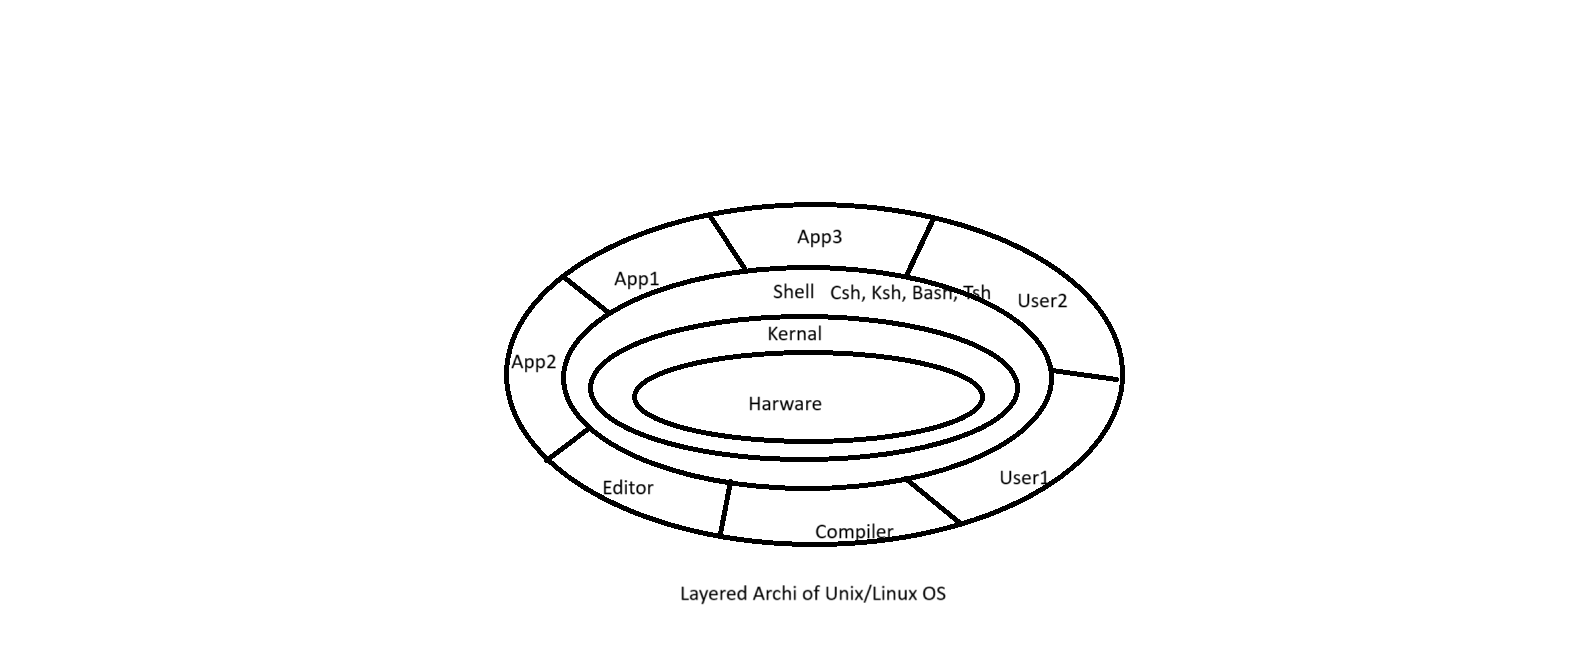
\includegraphics[keepaspectratio]{LinuxLayers.png}}

\begin{center}\rule{0.5\linewidth}{0.5pt}\end{center}

\subsection{\texorpdfstring{\textbf{📌 Linux File System
Basics}}{📌 Linux File System Basics}}\label{linux-file-system-basics}

📌 \textbf{Linux follows a hierarchical directory structure starting
from \texttt{/} (root).}

\begin{longtable}[]{@{}ll@{}}
\toprule\noalign{}
\textbf{Directory} & \textbf{Description} \\
\midrule\noalign{}
\endhead
\bottomrule\noalign{}
\endlastfoot
\texttt{/} & \textbf{Root directory} (Base of the filesystem) \\
\texttt{/bin} & User \textbf{binary files} (e.g., \texttt{ls},
\texttt{cp}, \texttt{mv}) \\
\texttt{/sbin} & System \textbf{binary files} (for admin tasks) \\
\texttt{/etc} & Configuration files for \textbf{system settings} \\
\texttt{/dev} & Stores device files (e.g., \texttt{/dev/sda} for
disks) \\
\texttt{/proc} & Virtual directory for \textbf{process information} \\
\texttt{/var} & Stores \textbf{logs, caches, and variable files} \\
\texttt{/tmp} & Temporary files (deleted on reboot) \\
\texttt{/usr} & User-related programs and libraries \\
\texttt{/home} & \textbf{User home directories}
(\texttt{/home/user1}) \\
\texttt{/boot} & Bootloader files for starting Linux \\
\texttt{/opt} & Optional software packages \\
\texttt{/lib} & System libraries required for OS functionality \\
\end{longtable}

\begin{center}\rule{0.5\linewidth}{0.5pt}\end{center}

\subsection{\texorpdfstring{\textbf{📌 Important Linux
Commands}}{📌 Important Linux Commands}}\label{important-linux-commands}

Linux is primarily controlled via the \textbf{command line (CLI)}.

📌 \textbf{File \& Directory Management Commands:}\\
✅ \texttt{pwd} → Print the \textbf{current working directory}.\\
✅ \texttt{ls} → List \textbf{files and directories}.\\
✅ \texttt{nano\ \textless{}file\textgreater{}} → Open the \textbf{nano
text editor}.\\
✅ \texttt{touch\ \textless{}file\textgreater{}} → Create a \textbf{new
file}.\\
✅ \texttt{mkdir\ \textless{}dir\textgreater{}} → Create a \textbf{new
directory}.\\
✅ \texttt{rm\ \textless{}file\textgreater{}} → Remove a
\textbf{file}.\\
✅ \texttt{rmdir\ \textless{}dir\textgreater{}} → Remove an
\textbf{empty directory}.\\
✅ \texttt{cd\ \textless{}dir\textgreater{}} → Change the
\textbf{current directory}.\\
✅ \texttt{chmod\ 755\ file} → Change \textbf{file permissions}.\\
✅ \texttt{chown\ user:group\ file} → Change \textbf{file ownership}.

📌 \textbf{Illustration:}\\
\pandocbounded{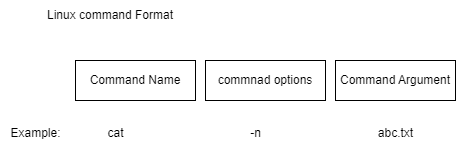
\includegraphics[keepaspectratio]{Day_2_6.png}}

\begin{center}\rule{0.5\linewidth}{0.5pt}\end{center}

\subsection{\texorpdfstring{\textbf{📌 What is a Shell in
Linux?}}{📌 What is a Shell in Linux?}}\label{what-is-a-shell-in-linux}

📌 \textbf{The Shell is an interface between the user and the Linux
kernel.}

✔ \textbf{It takes user commands, interprets them, and sends them to the
OS for execution.}\\
✔ \textbf{Users can interact with the shell via terminal commands or
shell scripts.}

📌 \textbf{Types of Shells in Linux:}

\begin{longtable}[]{@{}
  >{\raggedright\arraybackslash}p{(\linewidth - 4\tabcolsep) * \real{0.3333}}
  >{\raggedright\arraybackslash}p{(\linewidth - 4\tabcolsep) * \real{0.3333}}
  >{\raggedright\arraybackslash}p{(\linewidth - 4\tabcolsep) * \real{0.3333}}@{}}
\toprule\noalign{}
\begin{minipage}[b]{\linewidth}\raggedright
\textbf{Shell Type}
\end{minipage} & \begin{minipage}[b]{\linewidth}\raggedright
\textbf{Path}
\end{minipage} & \begin{minipage}[b]{\linewidth}\raggedright
\textbf{Description}
\end{minipage} \\
\midrule\noalign{}
\endhead
\bottomrule\noalign{}
\endlastfoot
\textbf{Bourne Shell (sh)} & \texttt{/bin/sh} & The \textbf{original
Unix shell} \\
\textbf{Bash (Bourne Again Shell)} & \texttt{/bin/bash} & Most commonly
used \textbf{default Linux shell} \\
\textbf{Restricted Bash (rbash)} & \texttt{/bin/rbash} & A limited
version of Bash \\
\textbf{Dash} & \texttt{/bin/dash} & A \textbf{lightweight shell},
faster than Bash \\
\textbf{Tmux} & \texttt{/usr/bin/tmux} & A terminal multiplexer \\
\textbf{Screen} & \texttt{/usr/bin/screen} & Allows \textbf{multiple
terminal sessions} \\
\end{longtable}

\begin{center}\rule{0.5\linewidth}{0.5pt}\end{center}

\subsection{\texorpdfstring{\textbf{📌 Shell
Variables}}{📌 Shell Variables}}\label{shell-variables}

📌 \textbf{Shell variables store values for use in scripts.}

✔ Can store \textbf{strings, numbers, and command outputs}.\\
✔ No need to specify \textbf{variable types}.

📌 \textbf{Example:}

\begin{Shaded}
\begin{Highlighting}[]
\VariableTok{X}\OperatorTok{=}\NormalTok{100      }\CommentTok{\# Assigns 100 to variable X}
\VariableTok{Y}\OperatorTok{=}\StringTok{"Linux"}  \CommentTok{\# Assigns "Linux" to variable Y}

\BuiltInTok{echo} \VariableTok{$X}    \CommentTok{\# Prints 100}
\BuiltInTok{echo} \VariableTok{$Y}    \CommentTok{\# Prints Linux}
\end{Highlighting}
\end{Shaded}

📌 \textbf{Reading Input in Shell Scripts:}

\begin{Shaded}
\begin{Highlighting}[]
\BuiltInTok{echo} \StringTok{"Enter your name:"}
\BuiltInTok{read} \VariableTok{name}
\BuiltInTok{echo} \StringTok{"Hello, }\VariableTok{$name}\StringTok{!"}
\end{Highlighting}
\end{Shaded}

📌 \textbf{Printing Output:}

\begin{Shaded}
\begin{Highlighting}[]
\BuiltInTok{echo} \StringTok{"This is a Linux script!"}
\end{Highlighting}
\end{Shaded}

\begin{center}\rule{0.5\linewidth}{0.5pt}\end{center}

\subsection{\texorpdfstring{\textbf{📌 Operators in
Linux}}{📌 Operators in Linux}}\label{operators-in-linux}

\subsubsection{\texorpdfstring{\textbf{1️⃣ Redirection Operators
(\texttt{\textgreater{}}, \texttt{\textgreater{}\textgreater{}},
\texttt{\textless{}})}}{1️⃣ Redirection Operators (\textgreater, \textgreater\textgreater, \textless)}}\label{redirection-operators}

📌 \textbf{Used to redirect input/output.}

✔ \texttt{\textgreater{}} → Overwrites a file\\
✔ \texttt{\textgreater{}\textgreater{}} → Appends to a file\\
✔ \texttt{\textless{}} → Takes input from a file

📌 \textbf{Example:}

\begin{Shaded}
\begin{Highlighting}[]
\BuiltInTok{echo} \StringTok{"Hello World"} \OperatorTok{\textgreater{}}\NormalTok{ file.txt  }\CommentTok{\# Creates file.txt and writes "Hello World"}
\BuiltInTok{echo} \StringTok{"Another Line"} \OperatorTok{\textgreater{}\textgreater{}}\NormalTok{ file.txt  }\CommentTok{\# Appends "Another Line" to file.txt}
\FunctionTok{cat} \OperatorTok{\textless{}}\NormalTok{ file.txt  }\CommentTok{\# Reads contents of file.txt}
\end{Highlighting}
\end{Shaded}

\subsubsection{\texorpdfstring{\textbf{2️⃣ Pipe Operator
(\texttt{\textbar{}})}}{2️⃣ Pipe Operator (\textbar)}}\label{pipe-operator}

📌 \textbf{Used to pass output of one command as input to another.}

📌 \textbf{Example:}

\begin{Shaded}
\begin{Highlighting}[]
\FunctionTok{cat}\NormalTok{ file.txt }\KeywordTok{|} \FunctionTok{grep} \StringTok{"error"}  \CommentTok{\# Finds "error" in file.txt}
\FunctionTok{ls} \AttributeTok{{-}l} \KeywordTok{|} \FunctionTok{less}  \CommentTok{\# Displays long list format in a paginated view}
\end{Highlighting}
\end{Shaded}

\begin{center}\rule{0.5\linewidth}{0.5pt}\end{center}

\subsection{\texorpdfstring{\textbf{📌 File Permissions \& Access
Control}}{📌 File Permissions \& Access Control}}\label{file-permissions-access-control}

📌 \textbf{Linux assigns three types of permissions to each file:}

\begin{itemize}
\tightlist
\item
  \textbf{Read (\texttt{r})} → View file contents.
\item
  \textbf{Write (\texttt{w})} → Modify file contents.
\item
  \textbf{Execute (\texttt{x})} → Run the file as a program.
\end{itemize}

📌 \textbf{File Permission Representation:}

\begin{verbatim}
-rwxr-xr--  1 user group  4096 Feb 25 10:00 file.txt
\end{verbatim}

📌 \textbf{Breakdown of Permissions:}

\begin{longtable}[]{@{}llll@{}}
\toprule\noalign{}
\textbf{Symbol} & \textbf{Owner} & \textbf{Group} & \textbf{Others} \\
\midrule\noalign{}
\endhead
\bottomrule\noalign{}
\endlastfoot
\textbf{rwx} & Read, Write, Execute & Read, Execute & Read \\
\end{longtable}

📌 \textbf{Changing File Permissions:}

\begin{Shaded}
\begin{Highlighting}[]
\FunctionTok{chmod}\NormalTok{ 755 file.txt  }\CommentTok{\# Owner: rwx, Group: r{-}x, Others: r{-}x}
\FunctionTok{chmod}\NormalTok{ 644 file.txt  }\CommentTok{\# Owner: rw{-}, Group: r{-}{-}, Others: r{-}{-}}
\end{Highlighting}
\end{Shaded}

📌 \textbf{Changing File Ownership:}

\begin{Shaded}
\begin{Highlighting}[]
\FunctionTok{chown}\NormalTok{ user:group file.txt  }\CommentTok{\# Assigns ownership to user and group}
\end{Highlighting}
\end{Shaded}

\begin{center}\rule{0.5\linewidth}{0.5pt}\end{center}

\subsection{\texorpdfstring{\textbf{📌 Shell Programming
Basics}}{📌 Shell Programming Basics}}\label{shell-programming-basics}

📌 \textbf{Shell scripts automate repetitive tasks in Linux.}

\subsubsection{\texorpdfstring{\textbf{1️⃣ Conditional Statements
(\texttt{if-else})}}{1️⃣ Conditional Statements (if-else)}}\label{conditional-statements-if-else}

\begin{Shaded}
\begin{Highlighting}[]
\ControlFlowTok{if} \BuiltInTok{[} \VariableTok{$X} \OtherTok{{-}gt}\NormalTok{ 10 }\BuiltInTok{]}
\ControlFlowTok{then}
  \BuiltInTok{echo} \StringTok{"X is greater than 10"}
\ControlFlowTok{else}
  \BuiltInTok{echo} \StringTok{"X is 10 or less"}
\ControlFlowTok{fi}
\end{Highlighting}
\end{Shaded}

\subsubsection{\texorpdfstring{\textbf{2️⃣ Loops in Shell
Scripts}}{2️⃣ Loops in Shell Scripts}}\label{loops-in-shell-scripts}

\paragraph{\texorpdfstring{\textbf{For Loop}}{For Loop}}\label{for-loop}

\begin{Shaded}
\begin{Highlighting}[]
\ControlFlowTok{for}\NormalTok{ i }\KeywordTok{in}\NormalTok{ 1 2 3 4 5}
\ControlFlowTok{do}
  \BuiltInTok{echo} \StringTok{"Iteration }\VariableTok{$i}\StringTok{"}
\ControlFlowTok{done}
\end{Highlighting}
\end{Shaded}

\paragraph{\texorpdfstring{\textbf{While
Loop}}{While Loop}}\label{while-loop}

\begin{Shaded}
\begin{Highlighting}[]
\VariableTok{X}\OperatorTok{=}\NormalTok{1}
\ControlFlowTok{while} \BuiltInTok{[} \VariableTok{$X} \OtherTok{{-}le}\NormalTok{ 5 }\BuiltInTok{]}
\ControlFlowTok{do}
  \BuiltInTok{echo} \StringTok{"Loop iteration: }\VariableTok{$X}\StringTok{"}
  \VariableTok{X}\OperatorTok{=}\VariableTok{$((X} \OperatorTok{+} \DecValTok{1}\VariableTok{))}
\ControlFlowTok{done}
\end{Highlighting}
\end{Shaded}

\begin{center}\rule{0.5\linewidth}{0.5pt}\end{center}

\subsection{\texorpdfstring{\textbf{📌 To Be Discussed Tomorrow Evening
(27-02-2025)}}{📌 To Be Discussed Tomorrow Evening (27-02-2025)}}\label{to-be-discussed-tomorrow-evening-27-02-2025}

📌 \textbf{Advanced Linux Topics:}\\
✅ \textbf{Advanced Operators (Redirection, Pipe, etc.)}\\
✅ \textbf{File Permissions \& Access Control Lists}\\
✅ \textbf{More Shell Programming -- Wildcards, Regular Expressions}\\
✅ \textbf{Command Line Arguments in Shell Scripts}\\
✅ \textbf{Decision Loops (if-else, case, while, for, until)}\\
✅ \textbf{Arithmetic Expressions \& Shell Scripting Examples}

\section{\texorpdfstring{\textbf{OS Notes -- Day
3}}{OS Notes -- Day 3}}\label{os-notes-day-3}

📅 \textbf{Date:} 27-02-2025

\begin{longtable}[]{@{}
  >{\raggedright\arraybackslash}p{(\linewidth - 0\tabcolsep) * \real{0.0556}}@{}}
\toprule\noalign{}
\begin{minipage}[b]{\linewidth}\raggedright
session 1
\end{minipage} \\
\midrule\noalign{}
\endhead
\bottomrule\noalign{}
\endlastfoot
\# \textbf{Memory Hierarchy -- Detailed Explanation} \\
\#\# \textbf{📌 What is Memory Hierarchy?} \\
Memory hierarchy is the \textbf{structured arrangement of memory
components} in a computer system, organized to \textbf{optimize speed,
cost, and capacity}. \\
📌 \textbf{Key Idea:} \\
- \textbf{Faster memories are expensive \& small}, while \textbf{slower
memories are cheaper \& large}. - \textbf{Frequently used data is stored
in faster memory} (Registers, Cache). - \textbf{Less frequently used
data is stored in slower memory} (RAM, Disk). \\
📌 \textbf{Illustration of Memory Hierarchy:} \\
\texttt{⬆\ Faster\ Access,\ Lower\ Capacity,\ Higher\ Cost\ ───────────────────────────────────\ \textbar{}\ \ Registers\ \ \ \textbar{}\ \ (Inside\ CPU,\ Fastest,\ Smallest)\ \textbar{}\ \textbar{}\ \ Cache\ (L1,\ L2,\ L3)\ \textbar{}\ \ (Fast,\ Stores\ Recent\ Data)\ \textbar{}\ \textbar{}\ \ Main\ Memory\ (RAM)\ \ \textbar{}\ \ (Larger\ but\ Slower)\ \textbar{}\ \textbar{}\ \ Secondary\ Storage\ \ \textbar{}\ \ (Hard\ Drive,\ SSD,\ Persistent)\ \textbar{}\ \textbar{}\ \ Tertiary\ Storage\ \ \ \textbar{}\ \ (Cloud,\ Magnetic\ Tape)\ \textbar{}\ ───────────────────────────────────\ ⬇\ Slower\ Access,\ Higher\ Capacity,\ Lower\ Cost} \\
\end{longtable}

\subsection{\texorpdfstring{\textbf{📌 Levels of Memory
Hierarchy}}{📌 Levels of Memory Hierarchy}}\label{levels-of-memory-hierarchy}

\subsubsection{\texorpdfstring{\textbf{1️⃣ Registers} (Fastest, Inside
CPU)}{1️⃣ Registers (Fastest, Inside CPU)}}\label{registers-fastest-inside-cpu}

✔ \textbf{Location:} Inside the CPU.\\
✔ \textbf{Characteristics:}

\begin{itemize}
\tightlist
\item
  Fastest memory, directly accessible by the CPU.
\item
  Limited number (usually 32 or 64 registers per CPU).
\item
  Stores temporary data for arithmetic/logical operations.\\
  ✔ \textbf{Use:} Holds the \textbf{operands and results} of CPU
  instructions.
\end{itemize}

📌 \textbf{Example:}

\begin{itemize}
\tightlist
\item
  When executing \texttt{A\ +\ B}, values of \texttt{A} and \texttt{B}
  are stored in registers for quick addition.
\end{itemize}

\begin{center}\rule{0.5\linewidth}{0.5pt}\end{center}

\subsubsection{\texorpdfstring{\textbf{2️⃣ Cache Memory} (High-Speed
Buffer)}{2️⃣ Cache Memory (High-Speed Buffer)}}\label{cache-memory-high-speed-buffer}

✔ \textbf{Purpose:} \textbf{Acts as a bridge between CPU and RAM} to
reduce access time.\\
✔ \textbf{Types of Cache:}

\begin{itemize}
\tightlist
\item
  \textbf{L1 (Level 1) Cache} → Fastest but \textbf{smallest}, located
  inside the CPU core.
\item
  \textbf{L2 (Level 2) Cache} → \textbf{Larger than L1}, but slightly
  slower.
\item
  \textbf{L3 (Level 3) Cache} → \textbf{Shared among multiple CPU
  cores}, improves multitasking.\\
  ✔ \textbf{Characteristics:}
\item
  \textbf{Stores frequently accessed data} to reduce memory access time.
\item
  Works based on \textbf{locality principles}:

  \begin{itemize}
  \tightlist
  \item
    \textbf{Temporal Locality:} Recently used data is likely to be used
    again soon.
  \item
    \textbf{Spatial Locality:} Data near recently used data is likely to
    be accessed soon.
  \end{itemize}
\end{itemize}

📌 \textbf{Example:}

\begin{itemize}
\tightlist
\item
  If a program frequently accesses an array, cache stores \textbf{nearby
  elements} to speed up access.
\end{itemize}

\begin{center}\rule{0.5\linewidth}{0.5pt}\end{center}

\subsubsection{\texorpdfstring{\textbf{3️⃣ Main Memory (RAM - Random
Access
Memory)}}{3️⃣ Main Memory (RAM - Random Access Memory)}}\label{main-memory-ram---random-access-memory}

✔ \textbf{Purpose:} Stores \textbf{active processes and data} for quick
CPU access.\\
✔ \textbf{Characteristics:}

\begin{itemize}
\tightlist
\item
  Larger capacity than Cache, but \textbf{slower}.
\item
  \textbf{Volatile} (Data lost when power is off).\\
  ✔ \textbf{Use:} Holds \textbf{running programs, operating system}, and
  \textbf{frequently accessed data}.
\end{itemize}

📌 \textbf{Example:}

\begin{itemize}
\tightlist
\item
  When opening an application (e.g., MS Word), it is \textbf{loaded from
  disk into RAM} for faster access.
\end{itemize}

\begin{center}\rule{0.5\linewidth}{0.5pt}\end{center}

\subsubsection{\texorpdfstring{\textbf{4️⃣ Secondary Storage (Hard Drive
\&
SSDs)}}{4️⃣ Secondary Storage (Hard Drive \& SSDs)}}\label{secondary-storage-hard-drive-ssds}

✔ \textbf{Purpose:} \textbf{Permanent storage} for files, programs, and
the OS.\\
✔ \textbf{Examples:} \textbf{Hard Disk Drives (HDDs), Solid-State Drives
(SSDs)}.\\
✔ \textbf{Characteristics:}

\begin{itemize}
\tightlist
\item
  \textbf{Non-volatile} (Retains data after shutdown).
\item
  Much \textbf{larger capacity than RAM}.
\item
  \textbf{Slower than RAM} but \textbf{cheaper per GB}.
\end{itemize}

📌 \textbf{Example:}

\begin{itemize}
\tightlist
\item
  When you save a file, it is \textbf{written to the hard disk} instead
  of RAM for long-term storage.
\end{itemize}

📌 \textbf{Comparison: HDD vs.~SSD}

\begin{longtable}[]{@{}
  >{\raggedright\arraybackslash}p{(\linewidth - 4\tabcolsep) * \real{0.3333}}
  >{\raggedright\arraybackslash}p{(\linewidth - 4\tabcolsep) * \real{0.3333}}
  >{\raggedright\arraybackslash}p{(\linewidth - 4\tabcolsep) * \real{0.3333}}@{}}
\toprule\noalign{}
\begin{minipage}[b]{\linewidth}\raggedright
\textbf{Feature}
\end{minipage} & \begin{minipage}[b]{\linewidth}\raggedright
\textbf{HDD (Hard Disk Drive)}
\end{minipage} & \begin{minipage}[b]{\linewidth}\raggedright
\textbf{SSD (Solid-State Drive)}
\end{minipage} \\
\midrule\noalign{}
\endhead
\bottomrule\noalign{}
\endlastfoot
\textbf{Speed} & Slower & Much Faster \\
\textbf{Durability} & Less Durable (Moving Parts) & More Durable (No
Moving Parts) \\
\textbf{Cost} & Cheaper per GB & More Expensive per GB \\
\end{longtable}

\begin{center}\rule{0.5\linewidth}{0.5pt}\end{center}

\subsubsection{\texorpdfstring{\textbf{5️⃣ Tertiary/External
Storage}}{5️⃣ Tertiary/External Storage}}\label{tertiaryexternal-storage}

✔ \textbf{Purpose:} \textbf{Backup, Archival, and Rarely Accessed
Data}.\\
✔ \textbf{Examples:} \textbf{Magnetic Tape, Optical Discs (CD/DVD),
Cloud Storage}.\\
✔ \textbf{Characteristics:}

\begin{itemize}
\tightlist
\item
  \textbf{Very high capacity}, but \textbf{slowest access speed}.
\item
  Used for \textbf{long-term storage} or \textbf{disaster recovery}.
\end{itemize}

📌 \textbf{Example:}

\begin{itemize}
\tightlist
\item
  \textbf{Magnetic tapes} store archived data in large data centers.
\item
  \textbf{Cloud storage (Google Drive, Dropbox)} allows \textbf{off-site
  backups}.
\end{itemize}

\begin{center}\rule{0.5\linewidth}{0.5pt}\end{center}

\subsection{\texorpdfstring{\textbf{📌 Key
Takeaways}}{📌 Key Takeaways}}\label{key-takeaways}

✅ \textbf{Speed vs.~Cost Trade-off:}

\begin{itemize}
\tightlist
\item
  \textbf{Faster memory = More expensive, Smaller size}.
\item
  \textbf{Slower memory = Cheaper, Larger capacity}.
\end{itemize}

✅ \textbf{Why Use a Hierarchy?}

\begin{itemize}
\tightlist
\item
  \textbf{Registers are limited}, so we use Cache.
\item
  \textbf{Cache is expensive}, so we use RAM.
\item
  \textbf{RAM is volatile}, so we use HDD/SSD.
\item
  \textbf{HDD/SSD is slow}, so we use Cache again.
\end{itemize}

✅ \textbf{Locality Principles:}

\begin{itemize}
\tightlist
\item
  \textbf{Temporal Locality:} If data is used once, it is likely to be
  used again soon.
\item
  \textbf{Spatial Locality:} If data at a memory location is accessed,
  nearby memory locations are likely to be accessed next.
\end{itemize}

\begin{center}\rule{0.5\linewidth}{0.5pt}\end{center}

\subsection{\texorpdfstring{\textbf{📌 Real-World Analogy: Memory
Hierarchy as a Kitchen
Setup}}{📌 Real-World Analogy: Memory Hierarchy as a Kitchen Setup}}\label{real-world-analogy-memory-hierarchy-as-a-kitchen-setup}

Imagine a \textbf{chef cooking in a kitchen}:

\begin{longtable}[]{@{}
  >{\raggedright\arraybackslash}p{(\linewidth - 4\tabcolsep) * \real{0.3333}}
  >{\raggedright\arraybackslash}p{(\linewidth - 4\tabcolsep) * \real{0.3333}}
  >{\raggedright\arraybackslash}p{(\linewidth - 4\tabcolsep) * \real{0.3333}}@{}}
\toprule\noalign{}
\begin{minipage}[b]{\linewidth}\raggedright
\textbf{Memory Level}
\end{minipage} & \begin{minipage}[b]{\linewidth}\raggedright
\textbf{Kitchen Equivalent}
\end{minipage} & \begin{minipage}[b]{\linewidth}\raggedright
\textbf{Speed}
\end{minipage} \\
\midrule\noalign{}
\endhead
\bottomrule\noalign{}
\endlastfoot
\textbf{Registers} & Ingredients in chef's hands & 🚀 Fastest \\
\textbf{Cache Memory} & Ingredients on the kitchen counter & 🔥 Very
Fast \\
\textbf{RAM (Main Memory)} & Ingredients in the fridge & ⚡ Fast \\
\textbf{Hard Drive (HDD/SSD)} & Ingredients in a grocery store & ⏳
Slow \\
\textbf{Tertiary Storage (Backup)} & Ingredients stored in a warehouse &
🐌 Slowest \\
\end{longtable}

📌 \textbf{Key Idea:} The chef uses the fastest and closest memory
(Registers \& Cache) most often, while accessing the fridge (RAM) or
store (HDD) only when necessary.

\begin{center}\rule{0.5\linewidth}{0.5pt}\end{center}

\subsection{\texorpdfstring{\textbf{📌 Process Scheduling
Algorithms}}{📌 Process Scheduling Algorithms}}\label{process-scheduling-algorithms}

\section{\texorpdfstring{\textbf{Process Scheduling Algorithms --
Detailed
Explanation}}{Process Scheduling Algorithms -- Detailed Explanation}}\label{process-scheduling-algorithms-detailed-explanation}

Process scheduling algorithms determine \textbf{which process the CPU
executes next} from the ready queue. The goal is to optimize \textbf{CPU
utilization, minimize waiting time, and improve system responsiveness}.

\begin{center}\rule{0.5\linewidth}{0.5pt}\end{center}

\subsection{\texorpdfstring{\textbf{📌 1. Shortest Job First (SJF)
Scheduling}}{📌 1. Shortest Job First (SJF) Scheduling}}\label{shortest-job-first-sjf-scheduling}

📌 \textbf{Definition:}

\begin{itemize}
\tightlist
\item
  The CPU selects the \textbf{process with the smallest execution time
  (CPU burst)} first.
\item
  \textbf{Goal:} Minimizes \textbf{average waiting time}, making it the
  \textbf{optimal algorithm} in ideal conditions.
\end{itemize}

📌 \textbf{Key Characteristics:}\\
✅ \textbf{Best average waiting time} if all processes arrive at the
same time.\\
✅ \textbf{Works well for batch systems} where CPU burst times are
known.\\
❌ \textbf{Starvation Issue:} Longer processes \textbf{may wait
indefinitely} if shorter jobs keep arriving.

📌 \textbf{Two Types of SJF:}

\subsubsection{\texorpdfstring{\textbf{🔹 Non-Preemptive
SJF}}{🔹 Non-Preemptive SJF}}\label{non-preemptive-sjf}

\begin{itemize}
\tightlist
\item
  \textbf{Once a process starts execution, it runs until completion} (No
  interruptions).
\item
  \textbf{Use Case:} Best for batch systems with \textbf{predictable CPU
  bursts}.
\end{itemize}

📌 \textbf{Example -- Non-Preemptive SJF:}

\begin{longtable}[]{@{}
  >{\raggedright\arraybackslash}p{(\linewidth - 10\tabcolsep) * \real{0.1667}}
  >{\raggedright\arraybackslash}p{(\linewidth - 10\tabcolsep) * \real{0.1667}}
  >{\raggedright\arraybackslash}p{(\linewidth - 10\tabcolsep) * \real{0.1667}}
  >{\raggedright\arraybackslash}p{(\linewidth - 10\tabcolsep) * \real{0.1667}}
  >{\raggedright\arraybackslash}p{(\linewidth - 10\tabcolsep) * \real{0.1667}}
  >{\raggedright\arraybackslash}p{(\linewidth - 10\tabcolsep) * \real{0.1667}}@{}}
\toprule\noalign{}
\begin{minipage}[b]{\linewidth}\raggedright
Process
\end{minipage} & \begin{minipage}[b]{\linewidth}\raggedright
Arrival Time (AT)
\end{minipage} & \begin{minipage}[b]{\linewidth}\raggedright
Burst Time (BT)
\end{minipage} & \begin{minipage}[b]{\linewidth}\raggedright
Completion Time (CT)
\end{minipage} & \begin{minipage}[b]{\linewidth}\raggedright
Turnaround Time (TAT = CT - AT)
\end{minipage} & \begin{minipage}[b]{\linewidth}\raggedright
Waiting Time (WT = TAT - BT)
\end{minipage} \\
\midrule\noalign{}
\endhead
\bottomrule\noalign{}
\endlastfoot
P1 & 0 & 8 & 8 & 8 - 0 = 8 & 0 \\
P2 & 1 & 4 & 12 & 12 - 1 = 11 & 7 \\
P3 & 2 & 9 & 21 & 21 - 2 = 19 & 10 \\
\end{longtable}

📌 \textbf{Gantt Chart for Non-Preemptive SJF:}

\begin{verbatim}
| P2 | P1 | P3 |
0    4    12   21
\end{verbatim}

📌 \textbf{Avg Waiting Time (AWT) = (0+7+10)/3 = 5.67 ms}\\
📌 \textbf{Illustration:}\\
\pandocbounded{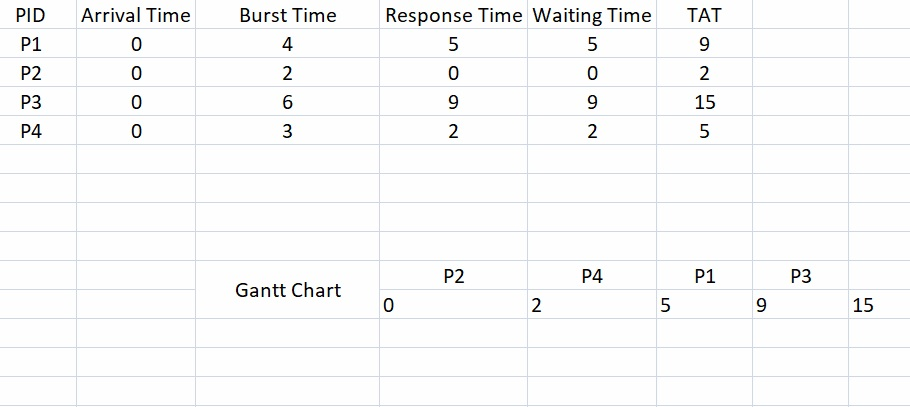
\includegraphics[keepaspectratio]{Day_3_1.jpg}}

\begin{center}\rule{0.5\linewidth}{0.5pt}\end{center}

\subsubsection{\texorpdfstring{\textbf{🔹 Preemptive SJF (Shortest
Remaining Time First -
SRTF)}}{🔹 Preemptive SJF (Shortest Remaining Time First - SRTF)}}\label{preemptive-sjf-shortest-remaining-time-first---srtf}

\begin{itemize}
\tightlist
\item
  \textbf{A new process can preempt the current running process if it
  has a shorter burst time.}
\item
  \textbf{Use Case:} Best for \textbf{time-sharing} or interactive
  systems.
\end{itemize}

📌 \textbf{Example -- Preemptive SJF (SRTF):}

\begin{longtable}[]{@{}
  >{\raggedright\arraybackslash}p{(\linewidth - 10\tabcolsep) * \real{0.1667}}
  >{\raggedright\arraybackslash}p{(\linewidth - 10\tabcolsep) * \real{0.1667}}
  >{\raggedright\arraybackslash}p{(\linewidth - 10\tabcolsep) * \real{0.1667}}
  >{\raggedright\arraybackslash}p{(\linewidth - 10\tabcolsep) * \real{0.1667}}
  >{\raggedright\arraybackslash}p{(\linewidth - 10\tabcolsep) * \real{0.1667}}
  >{\raggedright\arraybackslash}p{(\linewidth - 10\tabcolsep) * \real{0.1667}}@{}}
\toprule\noalign{}
\begin{minipage}[b]{\linewidth}\raggedright
Process
\end{minipage} & \begin{minipage}[b]{\linewidth}\raggedright
Arrival Time
\end{minipage} & \begin{minipage}[b]{\linewidth}\raggedright
Burst Time
\end{minipage} & \begin{minipage}[b]{\linewidth}\raggedright
Completion Time
\end{minipage} & \begin{minipage}[b]{\linewidth}\raggedright
Turnaround Time
\end{minipage} & \begin{minipage}[b]{\linewidth}\raggedright
Waiting Time
\end{minipage} \\
\midrule\noalign{}
\endhead
\bottomrule\noalign{}
\endlastfoot
P1 & 0 & 8 & 13 & 13 & 5 \\
P2 & 1 & 4 & 5 & 4 & 0 \\
P3 & 2 & 9 & 21 & 19 & 10 \\
\end{longtable}

📌 \textbf{Gantt Chart for Preemptive SJF (SRTF):}

\begin{verbatim}
| P2 | P1 | P3 |
1    5    13   21
\end{verbatim}

📌 \textbf{Avg Waiting Time (AWT) = 5.67 ms}\\
📌 \textbf{Illustration:}\\
\pandocbounded{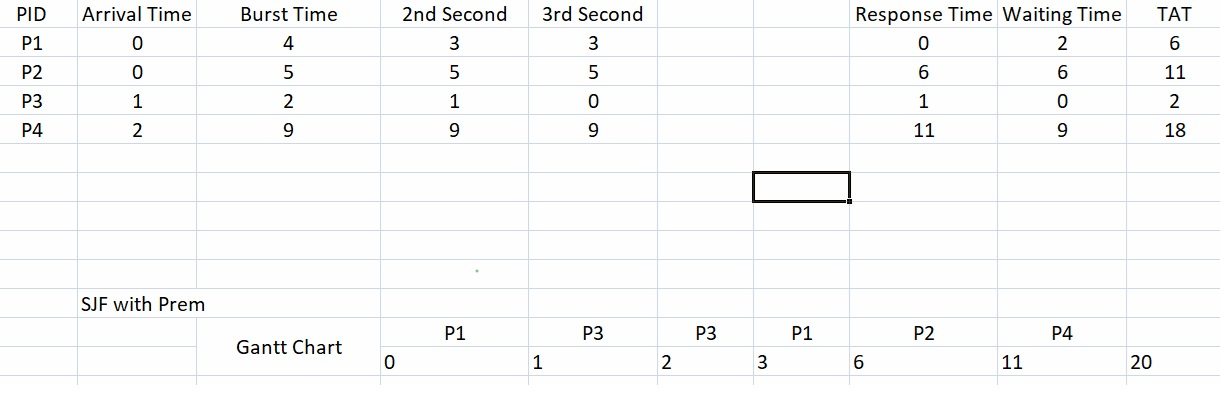
\includegraphics[keepaspectratio]{Day_3_4_SJF_Prem.jpg}}

\begin{center}\rule{0.5\linewidth}{0.5pt}\end{center}

\subsection{\texorpdfstring{\textbf{📌 2. Priority
Scheduling}}{📌 2. Priority Scheduling}}\label{priority-scheduling}

📌 \textbf{Definition:}

\begin{itemize}
\tightlist
\item
  \textbf{Each process is assigned a priority}, and the CPU selects the
  \textbf{highest-priority process} first.
\item
  \textbf{Priority can be static (fixed) or dynamic (changes over
  time).}
\end{itemize}

📌 \textbf{Key Characteristics:}\\
✅ \textbf{Ensures important tasks run first} (e.g., real-time OS).\\
✅ \textbf{Used in scheduling system processes.}\\
❌ \textbf{Starvation Issue:} Low-priority processes \textbf{may never
execute}.\\
✅ \textbf{Solution:} \textbf{Aging} (gradually increasing priority of
waiting processes).

📌 \textbf{Two Types of Priority Scheduling:}

\subsubsection{\texorpdfstring{\textbf{🔹 Preemptive Priority
Scheduling}}{🔹 Preemptive Priority Scheduling}}\label{preemptive-priority-scheduling}

\begin{itemize}
\tightlist
\item
  \textbf{A higher-priority process can interrupt a lower-priority
  running process.}
\item
  \textbf{Use Case:} \textbf{Real-time systems} (e.g., medical
  monitoring, airline systems).
\end{itemize}

\subsubsection{\texorpdfstring{\textbf{🔹 Non-Preemptive Priority
Scheduling}}{🔹 Non-Preemptive Priority Scheduling}}\label{non-preemptive-priority-scheduling}

\begin{itemize}
\tightlist
\item
  \textbf{A running process is not interrupted, even if a
  higher-priority process arrives.}
\item
  \textbf{Use Case:} Suitable for batch systems where tasks must
  \textbf{finish once started}.
\end{itemize}

📌 \textbf{Example -- Priority Scheduling:}

\begin{longtable}[]{@{}
  >{\raggedright\arraybackslash}p{(\linewidth - 12\tabcolsep) * \real{0.1429}}
  >{\raggedright\arraybackslash}p{(\linewidth - 12\tabcolsep) * \real{0.1429}}
  >{\raggedright\arraybackslash}p{(\linewidth - 12\tabcolsep) * \real{0.1429}}
  >{\raggedright\arraybackslash}p{(\linewidth - 12\tabcolsep) * \real{0.1429}}
  >{\raggedright\arraybackslash}p{(\linewidth - 12\tabcolsep) * \real{0.1429}}
  >{\raggedright\arraybackslash}p{(\linewidth - 12\tabcolsep) * \real{0.1429}}
  >{\raggedright\arraybackslash}p{(\linewidth - 12\tabcolsep) * \real{0.1429}}@{}}
\toprule\noalign{}
\begin{minipage}[b]{\linewidth}\raggedright
Process
\end{minipage} & \begin{minipage}[b]{\linewidth}\raggedright
Arrival Time
\end{minipage} & \begin{minipage}[b]{\linewidth}\raggedright
Burst Time
\end{minipage} & \begin{minipage}[b]{\linewidth}\raggedright
Priority
\end{minipage} & \begin{minipage}[b]{\linewidth}\raggedright
Completion Time
\end{minipage} & \begin{minipage}[b]{\linewidth}\raggedright
Turnaround Time
\end{minipage} & \begin{minipage}[b]{\linewidth}\raggedright
Waiting Time
\end{minipage} \\
\midrule\noalign{}
\endhead
\bottomrule\noalign{}
\endlastfoot
P1 & 0 & 8 & 2 & 8 & 8 & 0 \\
P2 & 1 & 4 & 1 & 5 & 4 & 0 \\
P3 & 2 & 9 & 3 & 21 & 19 & 10 \\
\end{longtable}

📌 \textbf{Gantt Chart for Priority Scheduling:}

\begin{verbatim}
| P2 | P1 | P3 |
1    5    13   22
\end{verbatim}

📌 \textbf{Avg Waiting Time (AWT) = 3.33 ms}\\
📌 \textbf{Illustration:}\\
\pandocbounded{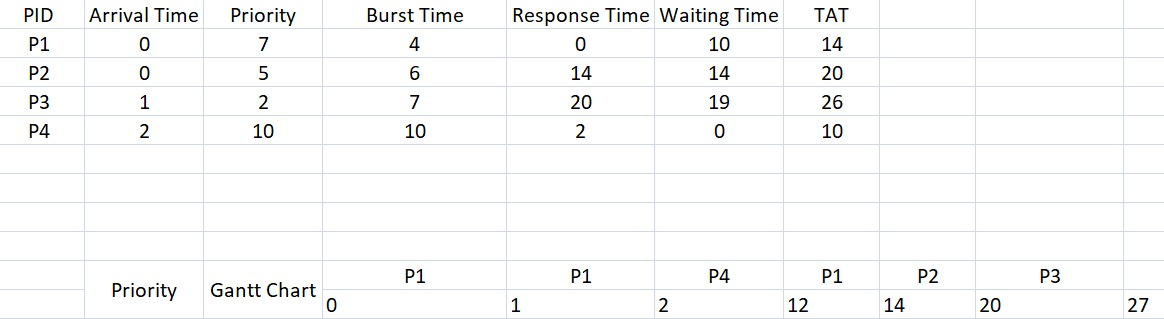
\includegraphics[keepaspectratio]{Day_3_5_Priority.jpg}}

\begin{center}\rule{0.5\linewidth}{0.5pt}\end{center}

\subsection{\texorpdfstring{\textbf{📌 3. Round Robin (RR)
Scheduling}}{📌 3. Round Robin (RR) Scheduling}}\label{round-robin-rr-scheduling}

📌 \textbf{Definition:}

\begin{itemize}
\tightlist
\item
  \textbf{Each process gets a fixed time slice (Time Quantum).}
\item
  \textbf{If a process doesn't finish within its time slice, it is moved
  to the back of the queue.}
\item
  \textbf{Used in multi-user and time-sharing systems.}
\end{itemize}

📌 \textbf{Key Characteristics:}\\
✅ \textbf{Fair Scheduling:} Every process \textbf{gets CPU time}.\\
✅ \textbf{Good for interactive systems.}\\
✅ \textbf{Ensures no process is starved.}\\
❌ \textbf{Too small a quantum = Too many context switches
(overhead).}\\
❌ \textbf{Too large a quantum = Behaves like FCFS.}

📌 \textbf{Example -- Round Robin (Time Quantum = 4 ms):}

\begin{longtable}[]{@{}
  >{\raggedright\arraybackslash}p{(\linewidth - 10\tabcolsep) * \real{0.1667}}
  >{\raggedright\arraybackslash}p{(\linewidth - 10\tabcolsep) * \real{0.1667}}
  >{\raggedright\arraybackslash}p{(\linewidth - 10\tabcolsep) * \real{0.1667}}
  >{\raggedright\arraybackslash}p{(\linewidth - 10\tabcolsep) * \real{0.1667}}
  >{\raggedright\arraybackslash}p{(\linewidth - 10\tabcolsep) * \real{0.1667}}
  >{\raggedright\arraybackslash}p{(\linewidth - 10\tabcolsep) * \real{0.1667}}@{}}
\toprule\noalign{}
\begin{minipage}[b]{\linewidth}\raggedright
Process
\end{minipage} & \begin{minipage}[b]{\linewidth}\raggedright
Arrival Time
\end{minipage} & \begin{minipage}[b]{\linewidth}\raggedright
Burst Time
\end{minipage} & \begin{minipage}[b]{\linewidth}\raggedright
Completion Time
\end{minipage} & \begin{minipage}[b]{\linewidth}\raggedright
Turnaround Time
\end{minipage} & \begin{minipage}[b]{\linewidth}\raggedright
Waiting Time
\end{minipage} \\
\midrule\noalign{}
\endhead
\bottomrule\noalign{}
\endlastfoot
P1 & 0 & 8 & 16 & 16 & 8 \\
P2 & 1 & 4 & 5 & 4 & 0 \\
P3 & 2 & 9 & 21 & 19 & 10 \\
\end{longtable}

📌 \textbf{Gantt Chart for Round Robin (Time Quantum = 4):}

\begin{verbatim}
| P1 | P2 | P3 | P1 | P3 |
0    4    8    12   16   21
\end{verbatim}

📌 \textbf{Avg Waiting Time (AWT) = 6 ms}\\
📌 \textbf{Illustration:}\\
\pandocbounded{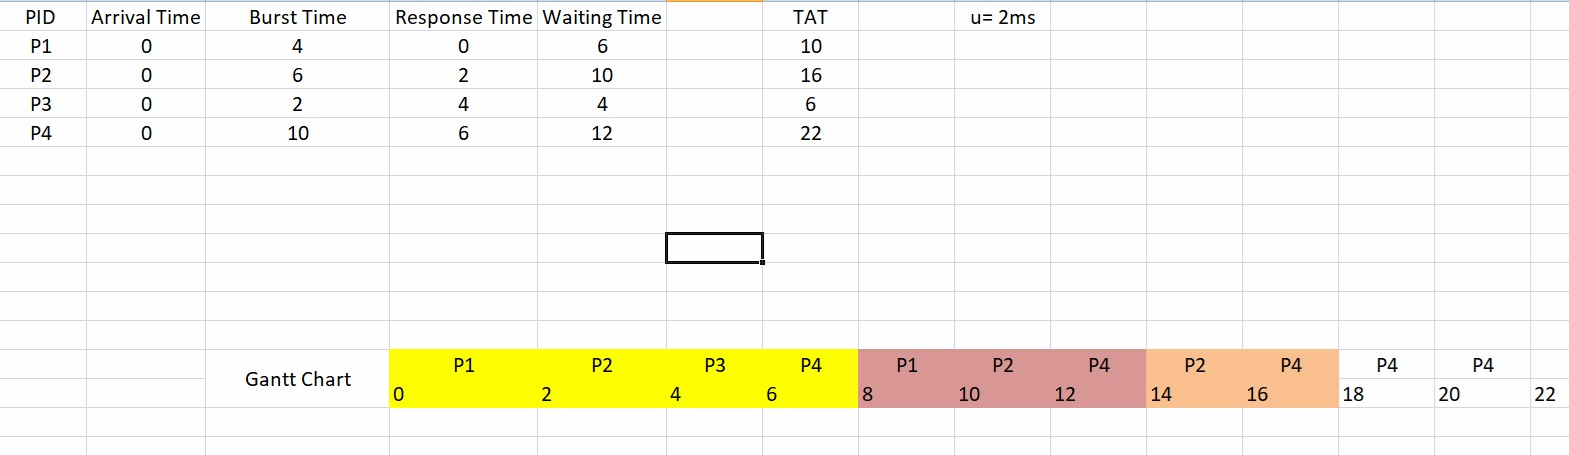
\includegraphics[keepaspectratio]{Day_3_2.jpg}}

\begin{center}\rule{0.5\linewidth}{0.5pt}\end{center}

\subsubsection{\texorpdfstring{\textbf{🔹 Impact of Reduced Quantum in
Round
Robin}}{🔹 Impact of Reduced Quantum in Round Robin}}\label{impact-of-reduced-quantum-in-round-robin}

📌 \textbf{If time quantum is too small, processes are switched too
frequently, causing high context-switching overhead.}

📌 \textbf{Example with Reduced Quantum:}\\
\pandocbounded{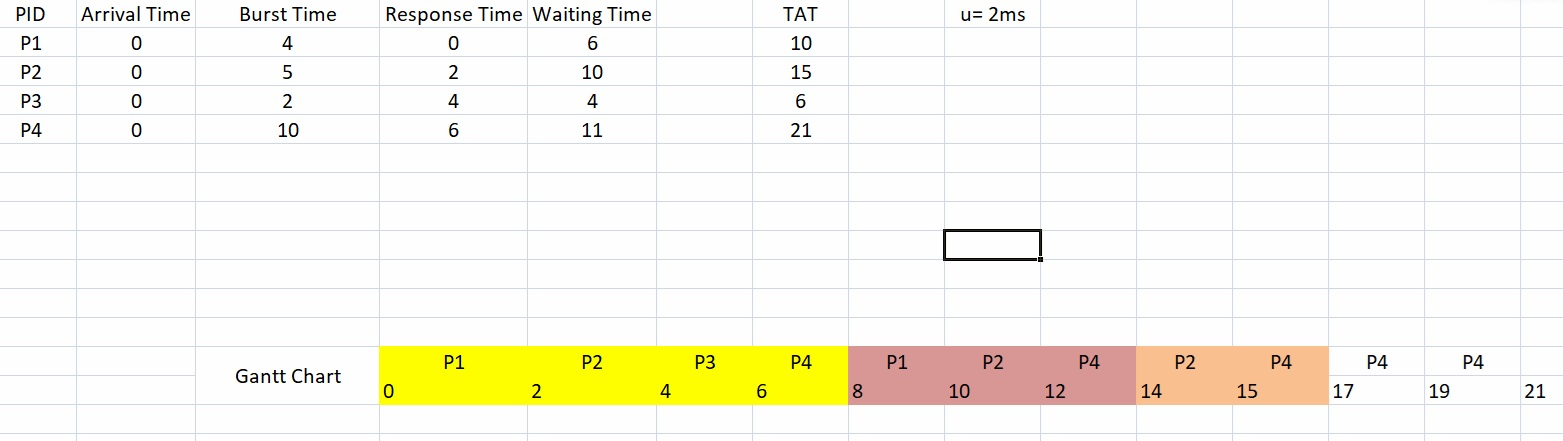
\includegraphics[keepaspectratio]{Day_3_3_RR_With_Reduced_Quantum.jpg}}

\begin{center}\rule{0.5\linewidth}{0.5pt}\end{center}

\subsection{\texorpdfstring{\textbf{📌 Summary of Scheduling
Algorithms}}{📌 Summary of Scheduling Algorithms}}\label{summary-of-scheduling-algorithms}

\begin{longtable}[]{@{}
  >{\raggedright\arraybackslash}p{(\linewidth - 8\tabcolsep) * \real{0.2000}}
  >{\raggedright\arraybackslash}p{(\linewidth - 8\tabcolsep) * \real{0.2000}}
  >{\raggedright\arraybackslash}p{(\linewidth - 8\tabcolsep) * \real{0.2000}}
  >{\raggedright\arraybackslash}p{(\linewidth - 8\tabcolsep) * \real{0.2000}}
  >{\raggedright\arraybackslash}p{(\linewidth - 8\tabcolsep) * \real{0.2000}}@{}}
\toprule\noalign{}
\begin{minipage}[b]{\linewidth}\raggedright
\textbf{Algorithm}
\end{minipage} & \begin{minipage}[b]{\linewidth}\raggedright
\textbf{Preemptive?}
\end{minipage} & \begin{minipage}[b]{\linewidth}\raggedright
\textbf{Optimal Waiting Time?}
\end{minipage} & \begin{minipage}[b]{\linewidth}\raggedright
\textbf{Starvation Risk?}
\end{minipage} & \begin{minipage}[b]{\linewidth}\raggedright
\textbf{Best For}
\end{minipage} \\
\midrule\noalign{}
\endhead
\bottomrule\noalign{}
\endlastfoot
\textbf{FCFS} & ❌ No & ❌ No & ✅ Yes (Long jobs delay short jobs) &
Simple batch processing \\
\textbf{SJF (Non-Preemptive)} & ❌ No & ✅ Yes & ✅ Yes (Starvation of
long jobs) & Ideal if burst time is known \\
\textbf{SJF (Preemptive - SRTF)} & ✅ Yes & ✅ Yes & ✅ Yes & Best for
multitasking \\
\textbf{Priority (Non-Preemptive)} & ❌ No & ❌ No & ✅ Yes & Used in
critical systems \\
\textbf{Priority (Preemptive)} & ✅ Yes & ❌ No & ✅ Yes & Real-time OS
(e.g., medical systems) \\
\textbf{Round Robin (RR)} & ✅ Yes & ❌ No & ❌ No & Time-sharing
systems \\
\end{longtable}

\begin{center}\rule{0.5\linewidth}{0.5pt}\end{center}

\subsection{\texorpdfstring{\textbf{📌 Key
Takeaways}}{📌 Key Takeaways}}\label{key-takeaways-1}

✔ \textbf{SJF minimizes average waiting time} but causes
\textbf{starvation}.\\
✔ \textbf{Priority Scheduling ensures important tasks run first} but can
cause \textbf{starvation}.\\
✔ \textbf{Round Robin guarantees fairness} but depends on
\textbf{quantum size}.\\
✔ \textbf{Choosing the best algorithm depends on system requirements.}

\begin{center}\rule{0.5\linewidth}{0.5pt}\end{center}

\subsection{\texorpdfstring{\textbf{📌 Memory
Hierarchy}}{📌 Memory Hierarchy}}\label{memory-hierarchy}

📌 \textbf{Definition:} A structured arrangement of different storage
types in a computer system, balancing \textbf{speed, cost, and
capacity}.

\subsubsection{\texorpdfstring{\textbf{Levels of Memory
Hierarchy}}{Levels of Memory Hierarchy}}\label{levels-of-memory-hierarchy-1}

\begin{longtable}[]{@{}
  >{\raggedright\arraybackslash}p{(\linewidth - 6\tabcolsep) * \real{0.2500}}
  >{\raggedright\arraybackslash}p{(\linewidth - 6\tabcolsep) * \real{0.2500}}
  >{\raggedright\arraybackslash}p{(\linewidth - 6\tabcolsep) * \real{0.2500}}
  >{\raggedright\arraybackslash}p{(\linewidth - 6\tabcolsep) * \real{0.2500}}@{}}
\toprule\noalign{}
\begin{minipage}[b]{\linewidth}\raggedright
\textbf{Memory Level}
\end{minipage} & \begin{minipage}[b]{\linewidth}\raggedright
\textbf{Characteristics}
\end{minipage} & \begin{minipage}[b]{\linewidth}\raggedright
\textbf{Speed}
\end{minipage} & \begin{minipage}[b]{\linewidth}\raggedright
\textbf{Size}
\end{minipage} \\
\midrule\noalign{}
\endhead
\bottomrule\noalign{}
\endlastfoot
\textbf{Registers} & Inside the CPU, extremely fast, very limited in
size & 🚀 Fastest & 🔹 Smallest \\
\textbf{Cache Memory (L1, L2, L3)} & Holds frequently accessed data to
speed up processing & 🚀 Very Fast & 🔹 Small \\
\textbf{Main Memory (RAM)} & Stores actively used data \& programs & ⚡
Fast & 🔹 Moderate \\
\textbf{Secondary Storage (HDD/SSD)} & Long-term storage (disk-based) &
⏳ Slower & 🔹 Large \\
\textbf{Tertiary Storage (Tape, Optical Disks)} & Used for backup \&
archives & 🐌 Slowest & 🔹 Very Large \\
\end{longtable}

📌 \textbf{Key Takeaways:}\\
✔ \textbf{Speed vs.~Cost Trade-off} → Faster memory is \textbf{more
expensive} per bit.\\
✔ \textbf{Locality Principle:}

\begin{itemize}
\tightlist
\item
  \textbf{Temporal Locality} → Recently accessed data is likely to be
  used again.
\item
  \textbf{Spatial Locality} → Nearby data is likely to be accessed soon.
\end{itemize}

\begin{center}\rule{0.5\linewidth}{0.5pt}\end{center}

\subsection{\texorpdfstring{\textbf{📌 Linux Useful Commands \& Shell
Scripting}}{📌 Linux Useful Commands \& Shell Scripting}}\label{linux-useful-commands-shell-scripting}

\subsubsection{\texorpdfstring{\textbf{🔹 Shell Scripting -- Decision
Loops}}{🔹 Shell Scripting -- Decision Loops}}\label{shell-scripting-decision-loops}

📌 \textbf{1️⃣ If-Else Statement}

\begin{Shaded}
\begin{Highlighting}[]
\ControlFlowTok{if} \BuiltInTok{[}\NormalTok{ condition }\BuiltInTok{]}
\ControlFlowTok{then}
    \ExtensionTok{statement}
\ControlFlowTok{else}
    \ExtensionTok{statement}
\ControlFlowTok{fi}
\end{Highlighting}
\end{Shaded}

📌 \textbf{Example:}

\begin{Shaded}
\begin{Highlighting}[]
\BuiltInTok{echo} \StringTok{"Enter a number:"}
\BuiltInTok{read} \VariableTok{num}
\ControlFlowTok{if} \BuiltInTok{[} \VariableTok{$num} \OtherTok{{-}eq}\NormalTok{ 5 }\BuiltInTok{]}
\ControlFlowTok{then}
    \BuiltInTok{echo} \StringTok{"Number is 5"}
\ControlFlowTok{else}
    \BuiltInTok{echo} \StringTok{"Number is not 5"}
\ControlFlowTok{fi}
\end{Highlighting}
\end{Shaded}

\begin{center}\rule{0.5\linewidth}{0.5pt}\end{center}

📌 \textbf{2️⃣ Nested If-Else}

\begin{Shaded}
\begin{Highlighting}[]
\ControlFlowTok{if} \BuiltInTok{[}\NormalTok{ condition }\BuiltInTok{]}
\ControlFlowTok{then}
    \ControlFlowTok{if} \BuiltInTok{[}\NormalTok{ condition }\BuiltInTok{]}
    \ControlFlowTok{then}
        \ExtensionTok{statement}
    \ControlFlowTok{else}
        \ExtensionTok{statement}
    \ControlFlowTok{fi}
\ControlFlowTok{else}
    \ControlFlowTok{if} \BuiltInTok{[}\NormalTok{ condition }\BuiltInTok{]}
    \ControlFlowTok{then}
        \ExtensionTok{statement}
    \ControlFlowTok{fi}
\ControlFlowTok{fi}
\end{Highlighting}
\end{Shaded}

📌 \textbf{Example:}

\begin{Shaded}
\begin{Highlighting}[]
\BuiltInTok{echo} \StringTok{"Enter three numbers:"}
\BuiltInTok{read} \VariableTok{num1} \VariableTok{num2} \VariableTok{num3}
\ControlFlowTok{if} \BuiltInTok{[} \VariableTok{$num1} \OtherTok{{-}gt} \VariableTok{$num2} \BuiltInTok{]}
\ControlFlowTok{then}
    \ControlFlowTok{if} \BuiltInTok{[} \VariableTok{$num1} \OtherTok{{-}gt} \VariableTok{$num3} \BuiltInTok{]}
    \ControlFlowTok{then}
        \BuiltInTok{echo} \StringTok{"}\VariableTok{$num1}\StringTok{ is the largest"}
    \ControlFlowTok{else}
        \BuiltInTok{echo} \StringTok{"}\VariableTok{$num3}\StringTok{ is the largest"}
    \ControlFlowTok{fi}
\ControlFlowTok{else}
    \ControlFlowTok{if} \BuiltInTok{[} \VariableTok{$num2} \OtherTok{{-}gt} \VariableTok{$num3} \BuiltInTok{]}
    \ControlFlowTok{then}
        \BuiltInTok{echo} \StringTok{"}\VariableTok{$num2}\StringTok{ is the largest"}
    \ControlFlowTok{else}
        \BuiltInTok{echo} \StringTok{"}\VariableTok{$num3}\StringTok{ is the largest"}
    \ControlFlowTok{fi}
\ControlFlowTok{fi}
\end{Highlighting}
\end{Shaded}

\begin{center}\rule{0.5\linewidth}{0.5pt}\end{center}

\subsubsection{\texorpdfstring{\textbf{🔹 Loops in Shell
Scripting}}{🔹 Loops in Shell Scripting}}\label{loops-in-shell-scripting}

📌 \textbf{1️⃣ For Loop} (Repeats code \textbf{n times})

\begin{Shaded}
\begin{Highlighting}[]
\ControlFlowTok{for}\NormalTok{ variable }\KeywordTok{in}\NormalTok{ value1 value2 value3}
\ControlFlowTok{do}
    \BuiltInTok{echo} \VariableTok{$variable}
\ControlFlowTok{done}
\end{Highlighting}
\end{Shaded}

📌 \textbf{Example:}

\begin{Shaded}
\begin{Highlighting}[]
\ControlFlowTok{for}\NormalTok{ num }\KeywordTok{in}\NormalTok{ 1 2 3 4 5}
\ControlFlowTok{do}
    \BuiltInTok{echo} \StringTok{"Number: }\VariableTok{$num}\StringTok{"}
\ControlFlowTok{done}
\end{Highlighting}
\end{Shaded}

📌 \textbf{Example with Sum Calculation:}

\begin{Shaded}
\begin{Highlighting}[]
\VariableTok{sum}\OperatorTok{=}\NormalTok{0}
\ControlFlowTok{for}\NormalTok{ num }\KeywordTok{in}\NormalTok{ 1 2 3 4 5}
\ControlFlowTok{do}
    \VariableTok{sum}\OperatorTok{=}\VariableTok{$((sum} \OperatorTok{+} \VariableTok{num))}
\ControlFlowTok{done}
\BuiltInTok{echo} \StringTok{"Sum is: }\VariableTok{$sum}\StringTok{"}
\end{Highlighting}
\end{Shaded}

\begin{center}\rule{0.5\linewidth}{0.5pt}\end{center}

\end{document}
